\chapter{Binding energy of the $^{86}$Sr$_2$ halo molecule} \label{ch:chap5}
%% ab initio calc are hard
Atomic interaction potentials are extremely difficult to predict \textit{a priori} for all but the simplest of atoms.
Despite this, the theoretical treatment of atomic collisions may be greatly simplified when describing dilute ultracold gases to a single parameter known as the $s$-wave scattering length, $a$.
The character of a dilute ultracold gas is one in which individual atoms are primarily in the long-range region relative to other atoms and their thermal energy is just above the $E=0$ threshold. 
%defined by the short-range interaction potential.
In this regime, the dominant interaction between atoms is the van der Waals interaction.
Ref.\,\cite{gfl93} subsequently demonstrated that a length scale, given by $\bar{a}=\frac{2 \pi}{\Gamma(1/4)^2} \left( \frac{2 \mu C_6}{\hbar^2} \right)^{1/4}$, may be defined that separates the short- and long-range portions of the potential.
Using this approximation, scattering and bound state wavefunctions may be constructed that relate the binding energy of the most weakly bound state in the potential to the $s$-wave scattering length \cite{fks96,gao04,Julienne2006}.
For $^{86}$Sr$_2$ the extremely small binding energy of the halo state is nearly entirely dependent on the behavior of the long-range van der Waals portion of the potential.

In the previous chapter, we explored the coupling of the intermediate state and halo state via measuring the halo molecule's susceptibility as a function of the light intensity and detuning from the intermediate state.
These measurements probed a strongly coupled regime and were found to produce large AC stark shifts and multi-photon Raman loss processes. 
To determine a precise value of the natural binding energy of the halo molecular state, we repeated similar experiments as before but with much lower excitation beam intensity at a fixed intermediate state detuning.

When describing two-photon spectroscopy to a weakly-bound ground state molecule, it is typical to neglect any potential AC Stark shift between the free ground state atoms and the bound state dimer caused by far off-resonant trapping lasers since the dimerized atoms contribute to the overall polarizability approximately as free atoms \cite{Jones2006}.
However, in general AC Stark shifts due to the trapping lasers and collisions with ground state atoms should also be considered to shift the molecular resonance as was taken into account in a recent, high-precision study of weakly bound molecular states of ultracold ytterbium atoms \cite{bbc17}.

% what we did in comparison to last chater
In this chapter, we accurately determine the $^{86}$Sr$_2$ halo state binding energy, considering possible collisional frequency shifts and AC Stark shifts due to trapping and excitation lasers.
Then using the universal prediction for the binding energy, including corrections derived for a van der Waals potential \cite{gfl93,Gao01,gao04}, we derive new estimates for the value of the strontium $C_6$ coefficient of the X$^1\Sigma_g^+$ potential from Ref.\,\cite{Stein2010}.
This modified version of the potential is then used to calculate improved scattering lengths for all strontium isotopes via mass scaling.

%We also varied the trap depth to look for any differences in susceptibility between the halo state and the asymptote.
%Efimov trimers also exist in systems near a scattering resonance, influencing dimer and atomic scattering properties and introducing additional universal phenomena \hl{\cite{bha07,nen17}}.
%In our first experiments probing the 86 halo, prsented in the previous chapter, we probed the regime of strong coupling and 
%These processes strongly perturbed the bare halo molecular state.
%and that our iniital experiments were in a strongly coupled regime
% what our results were
%% some good theory to characterize the long-range portion, binding energy of last state says a lot
%GF considered a pure van-der-waals C6 potential and found that it can be analytically solved for the binding energies by determining the phase factor?
%They then connected this to real potentials 
%By extending their model, they described interaction potentials that asymptote to a van-der-Waals form using an additional parameter, the van der Waals length $l_{\mathrm{vdW}}$, which defines a length scale beyond which the C6 portion of the potential dominates.
%This provided a way to estimate the binding energy for weakly bound molecular states.
%For system which exists near a scattering resonance, the analytic approximations of GF are expected to be quite accurate.
% $s$-wave scattering lengths and 
%we derive a more accurate value of the $s$-wave scattering length for $^{86}$Sr atomic collisions \hl{\cite{Stein10,mmp08}}.
%Using this binding energy we can compare to 
%say how we changed Eb2 from previous chapter
%The known scattering properties of strontium are mass scaled from 88 \hl{is this somehow not as good for 86? Also, where are the most up to date scattering lengths for Sr from?
%The '10 Fourier paper} but by probing the 86 ground state potential directly we can obtain a more accurate measurement of the 86-86 scattering length.
%\begin{equation}\label{Eq:GlobalFit}
%	E'_{b2}=E_{b2}+h\chi_{689}I_{689}+h\chi_{1064}I_{1064}(\mathbf{r})+h\chi_{n}n(\mathbf{r}).
%\end{equation}
%Recall that for an intermediate state detuning $\Delta_1/2 \pi = -9$\,MHz and low-intensity, then we are squarely in the raman regime.
%But the high precision of our measurement allows us to detect a small shift.
%This corresponds to a relative differential polarizability of ${\chi_{1064}}/{2\chi_{1064,\text{g}}g}={(\chi_{1064,b2}-2\chi_{1064,\text{g}}g}/{2\chi_{1064,\text{g}}g}\approx xx$.
%	\begin{figure} 
%	\centerline{
%	  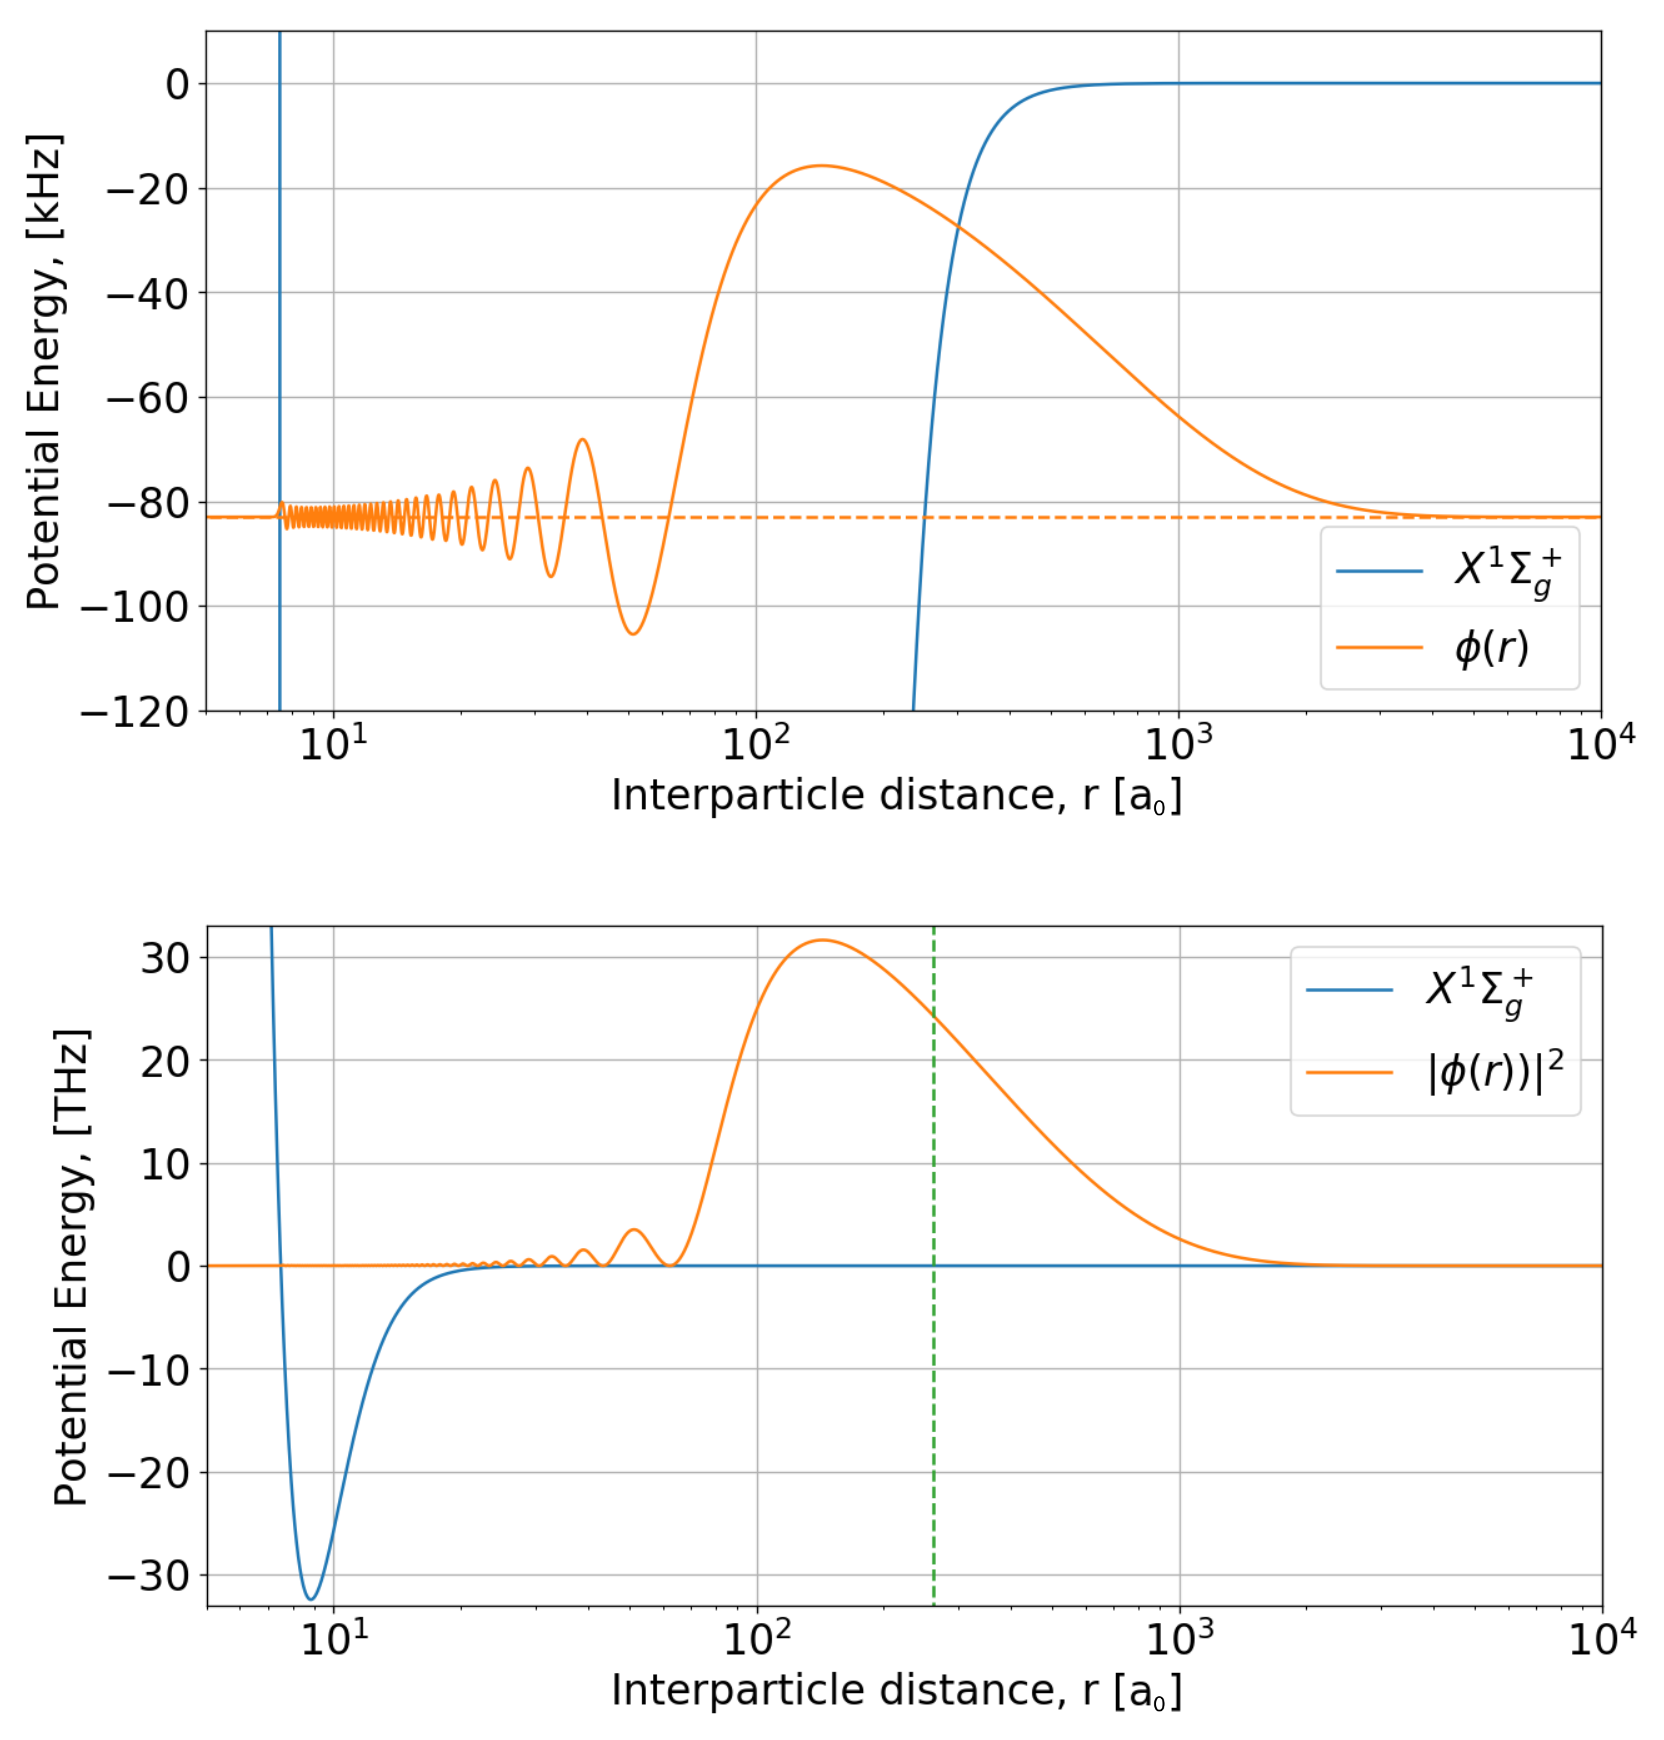
\includegraphics[width=\textwidth]{86halo.png}}
%	  \caption{$^{86}Sr$ halo molecule wavefunction}{The wavefunction (top) and probability amplitude (bottom) of the halo molecule calculated using the strontium ground state potential from Tiemann \hl{ref}. Note the difference in energy scales to illustrate the weakest portion of the ground state potential. The wavefunction and probability amplitude have been scaled to be visible on each figure and are not normalized. As expected the halo molecule extends far into the classically forbidden region with the classical turning point, given by Eq.\,\hl{something}, $r_{clas} = \left( \frac{a^2 m C_6}{\hbar^2} \right)^{1/6} \approx 260\,a_0$ }
%	  \label{fig:86haloWF}
%	\end{figure}

\section{Photoassociation in shallow traps} \label{sec:lowE_theory}
%%%% setup and differences
Excitation of the halo state proceeded using the same methodology as described in Sec.\,\ref{sec:highE_methods}, with the only difference being that the experiments reported here were performed in a single-beam optical dipole trap to produce a large trapping volume.
The trap is generated from a $1064\,\text{nm}$ laser that is aligned perpendicular to gravity with beam waists $260\,\mu\text{m}\,\times\,26\,\mu\text{m}$.
Following forced evaporation, typical atom numbers were several hundred thousand and typical atom temperatures were between $30\,\text{nK} - 1000\,\text{nK}$.
The atom number and sample temperature are measured using time-of-flight absorption imaging and trap oscillation frequencies are determined by measuring dipole and breathing collective mode frequencies.
These trap frequencies are confirmed against an independent model of the trapping potential.

The large volume of this single-beam optical trap allowed us to maintain peak densities $\approx\!\peakDens{1-2}{12}$, comparable to our previous work, over a range of various $1064$\,nm intensities.
For each trap intensity, two-photon spectroscopy was performed to search for a differential AC Stark shift at $1064\,\text{nm}$ between the free-atom asymptote of scattering states and the halo molecule state.

The experiments in the previous chapter revealed that photoassociation using high-intensity and/or large intermediate state detuning led to shifts of the halo molecular resonance that could not be explained by a simple three-level model.
In this study, the $689$\,nm excitation beam intensity was kept extremely low, such that the AC Stark shift remained proportional to $I_{689}$.
Additionally, the intermediate state detuning was fixed at $\Delta_1/2 \pi = -9$\,MHz.
Thus, these experiments are in the Raman regime with $\Delta_1 \gg \Omega_{12}$ and a theoretical description considering only a single intermediate state should be sufficient.


%%%% recap from before 
Loss spectra are modeled using the previously developed lineshape formulas of Bohn and Julienne, Sec.\,\ref{sec:highE_paLoss}.
Here we restate the main results needed for evaluating the current experiments.
\begingroup
\addtolength{\jot}{1em}
\begin{equation} \label{eq:chap5avgK}
	\langle K \rangle_\text{trap} = \frac{1}{V_2} \int_V e^{-2 U(\vec{r})/k_{B}T} \frac{1}{h\,Q_{T}} \int_{0}^{\epsilon_{\text{max}}(\vec{r})} d\epsilon \vert S(\epsilon, \vec{r}) \vert^2 \,e^{-\epsilon/k_{B}T}
\end{equation}
\begin{equation}\label{5equationApproxLorentzian}
  \vert S(\epsilon, \vec{r}) \vert^2 = \frac{\Gamma_L(\epsilon)+\gamma_{\text{eff}}}{\Gamma_L(\epsilon)} \frac{\eta  A(\epsilon)} {\left(\omega_1-\omega_2+\epsilon/\hbar-E'_{b2}(\vec{r})/\hbar\right)^2+\left[
  	\frac{\Gamma_L(\epsilon)+\gamma_{\text{eff}}}{2}\right]^2}
\end{equation}
\begin{align}
  A(\epsilon) &= \frac{\Omega_{12}^{4}\gamma_1 \gamma_s(\epsilon)}{16(\Delta_1+\epsilon/\hbar)^4} \\
  \Gamma_L(\epsilon) &= \frac{\Omega_{12}^{2}[\gamma_1 +\gamma_s(\epsilon)]}{4(\Delta_1+\epsilon/\hbar)^2}
\end{align}
\endgroup
The astute observer may notice that a subtle spatial dependence has been introduced into the collision energy distribution by an energy cutoff $\epsilon_{\text{max}}(\vec{r})$ defined by the local trap depth $\epsilon_{\text{max}}(\vec{r}) = U_{\text{depth}} - U(\vec{r})$.
The effect of this will be discussed momentarily.
Spatial dependence of the trapping laser intensity $I_{1064}(\vec{r})$ and the density $n(\vec{r})$ give rise to the spatial dependence of $\vert S(\epsilon, \vec{r}) \vert^2$ and the need for a spatial average in Eq.\,\ref{eq:chap5avgK}.
The $689$\,nm excitation beam is large compared to the atom sample so we neglect effects of spatial variation for this beam.

Recall from Sec.\,\ref{sssec:1064_modeling}, the trapping potential is given by $U(\mathbf{r})=mgz + \frac{\alpha(\lambda)}{2 \epsilon_0 c} I_{1064}(\mathbf{r})-\tilde{U}_{\text{min}}$, with $mgz$ the gravitational potential, $I_{1064}(\vec{r})$ the intensity of the trapping light, and $\alpha(\lambda)$ the polarizability of ground state atoms due to $1064$\,nm light.
Here we have subtracted off the trap minimum, $U_{\text{min}}$, such that the maximum kinetic energy of trapped particles is $U_{\text{depth}}$ as previously defined.
%Additionally, the scattering probability $\vert S(\epsilon, \vec{r}) \vert^2$, has been modified from it's usual formulation due to our consideration of the spatial dependence of $E'_{b2}(\vec{r})$.

The inclusion of a spatially dependent energy cutoff, $\epsilon_{\text{max}}(\vec{r})$, in Eq.\,\ref{eq:chap5avgK} is a result of the shallow trapping potentials used for these experiments.
Whether a trap is consider deep or shallow is determined by the ratio of trap depth to sample temperature, $\eta_{\text{trap}} = U_\text{depth}/k_B T$, where $\eta_{\text{trap}} \gtrsim 4$ is the approximate transition as will be shown in the next section.
The experiments in this chapter were performed in shallow traps where $\eta_\text{trap} \sim 1$ for the lowest temperature samples $T \approx 30$\,nK and $\eta_\text{trap} \sim 3$ for $T \approx 1000$\,nK\footnote{In the previous experiments at high-intensity, $\eta_\text{trap} > 6$ for all data, therefore a harmonic approximation was appropriately applied.}.

	\begin{figure} 
	\centerline{
	  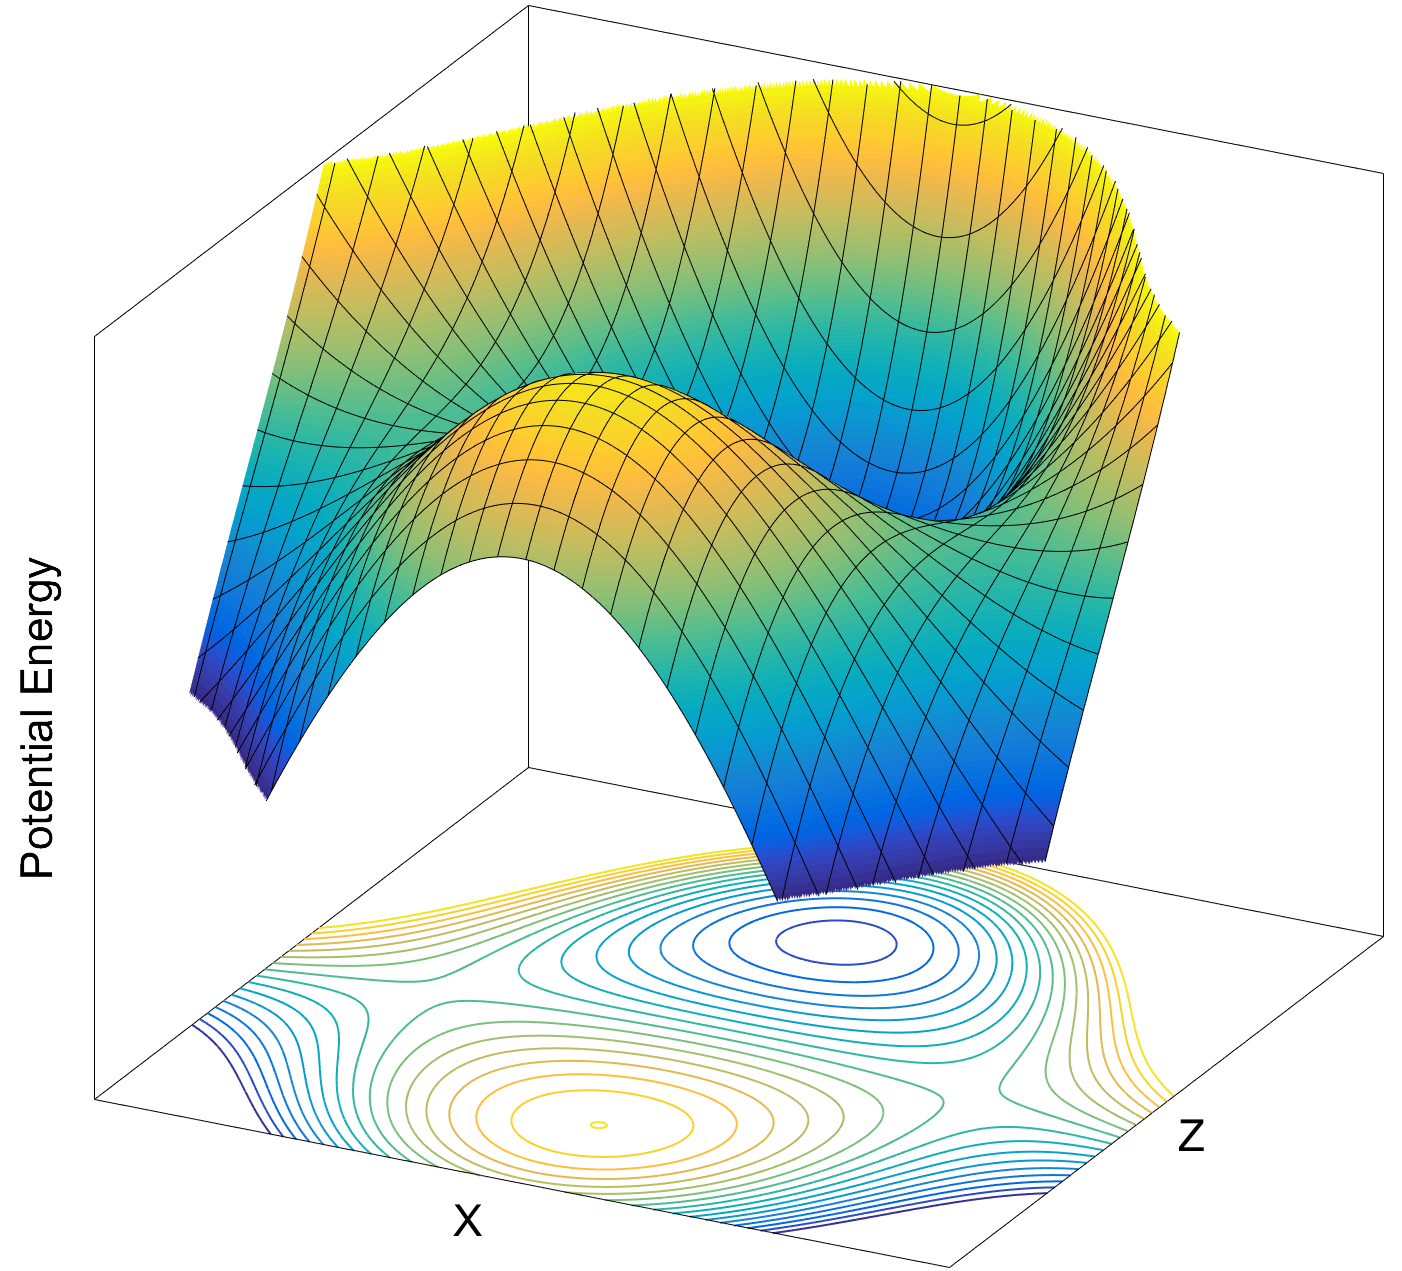
\includegraphics[width=\textwidth]{haloTrapV2.png}}
	  \caption{Surface plot of the trapping volume in single beam trap}{The spatial dependence along the $XZ$ plane with $Y=0$ of the ground state potential energy during the halo molecule excitation. Note, this coordinate system assumes the laser wavevector is propagating along $+X$ and gravity is aligned along $-Z$. We can clearly see the trap depth is defined along a trajectory where a particle is simultaneously moving away from the beam waist and down under the influence of gravity.}
	  \label{fig:haloTrapModel}
	\end{figure}
	
	\begin{figure} 
	\centerline{
	  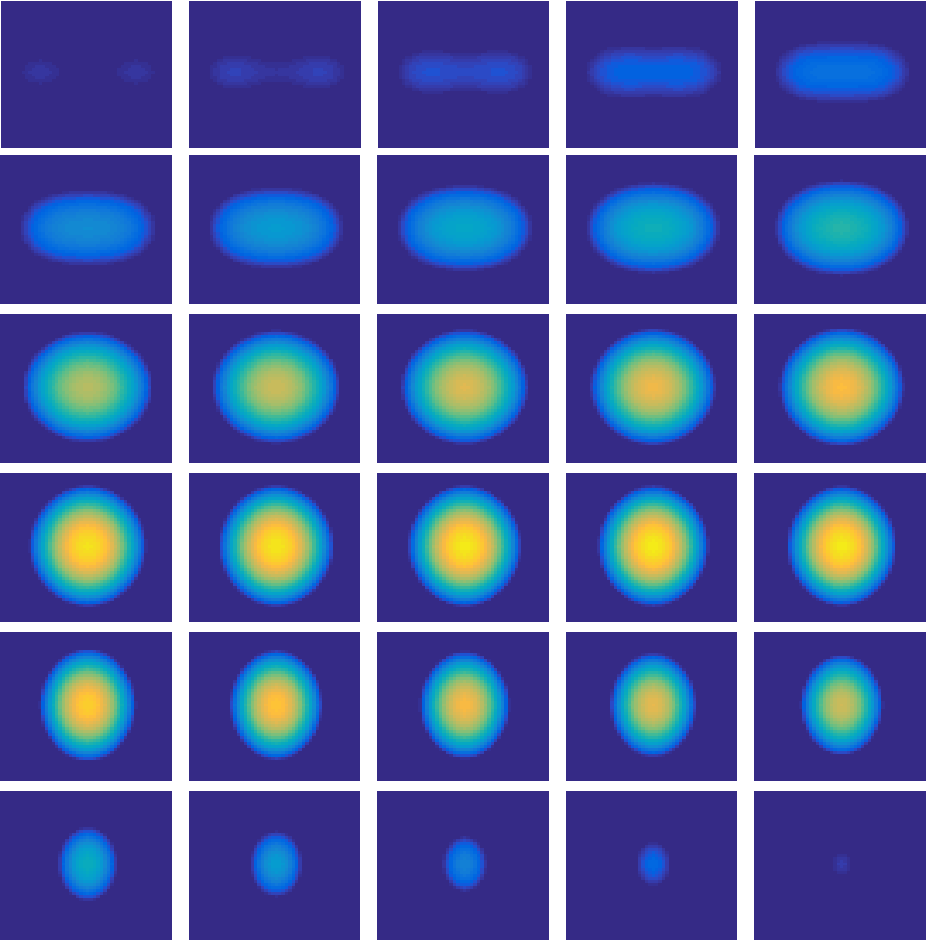
\includegraphics[height=0.5\textheight]{eta_over_space.png}}
	  \caption{Two-dimensional slices through single beam trap}{An alternative view of the potential shown in Fig.\,\ref{fig:haloTrapModel}. Each image is an $XY$ plane at a specific depth in $Z$. The first images start beneath the trap and continue to move up through the trapping region as the images progress left to right. All images share a common color scale where the deepest blue represents coordinates in space outside of the trapping region.}
	  \label{fig:halo2DTrapModel}
	\end{figure}
	
Since the harmonic approximation is not a valid description of the trapping potential in this regime, we instead use the full form of the Gaussian beam profile in our evaluation of $\langle K \rangle_\text{trap}$.
Fig.\,\ref{fig:haloTrapModel} shows a volumetric plot of a characteristic trapping potential used in the lowest temperature experiments where $\eta_\text{trap} \sim 1$.
From the plot, we can clearly identify a local maximum and the saddle point that defines $U_\text{depth}$.
This impacts equilibration in such a trap as the exit path lies along a non-trivial trajectory.
In real space, this trap appears as an elongated bowl in the $XY$ plane with a "hump" in the middle and small "funnels" on either end such that atoms must have low enough energy to fall under the influence of gravity along $-Z$ while simultaneously moving away from the trap center along $|X| > 0$, in order to find the minimum and exit.
This geometry is caused by the Gaussian nature of the extremely narrow vertical beam waist, $26\,\mu$m along the $Z$-axis.
The rapid expansion of the beam intensity in the vertical direction along the Rayleigh length, causes the trap to weaken along the $X$ direction quickly.

In addition to the abnormal trajectory required to leave the trap, atoms trapped in the central region near $X=0$ see a larger barrier to leaving the trap due to the local maximum.
Analysis of the trap revealed that this maximum is $\sim 2 \, U_\text{depth}$.
Thus atoms at kinetic energies higher than $U_\text{depth}$ may remain in the trapping region for a significant period of time before eventually finding a path to leave.
This suggests that our samples may have been out-of-equilibrium during the photoassociation process.

From Eq.\,\ref{eq:chap5avgK} and \ref{5equationApproxLorentzian}, we identify several factors which must be assessed for their spatial dependence when modeling photoassociation in a shallow trap.
These include $U(\vec{r})$, $\epsilon_\text{max}(\vec{r})$, and $E'_{b2}(\vec{r})$.
Given that we can determine $U(\vec{r})$ from beam parameters, we'll now consider the remaining two quantities.


\subsection{Effects of truncation on collision energy} \label{sec:trunc_trap}
Over the course of these experiments, we observed a slow rate of atom loss that was attributed to the large scattering length of $^{86}$Sr, $\sim40$\,nm, leading to three-body recombination or off-resonant scattering from the optical dipole trap.
Subsequent analysis of the trapping potential and PA spectra leads us to hypothesize that this atom loss was, at least partly, caused by the diminished thermalization rate expected in this irregular trap geometry.
Lacking a detailed microscopic model of the atomic density and momentum distribution in this shallow trap, we proceed by assuming the single-particle kinetic energy may be described by a truncated Maxwell-Boltzmann distribution such that energies above a particular cut-off, $\epsilon_\text{max}$, do not contribute to the scattering probability in the photoassociation process.
Furthermore, we assume the density does not change during the excitation time.
This is a reasonable assumption given that our exposure times were short compared to any background change in density and the sample temperature varied by no more than $15$\% for all values of $\Delta_2$.

%We consider the effects of truncation due to the extreme shallowness of the trap and the slow rate of thermalization observed over the course of these experiments.
%Due to the shallowness of the trap and the slow rate of thermalization observed during the experiments, we model the non-equilibrium kinetic energy distribution of the gas 

The equilibrium relative momentum distribution, $f(|\vec{p}_\text{R}|)$, of a gas of particles with reduced mass $\mu$ at temperature $T$, is given by a Maxwell-Boltzmann distribution.
A derivation of this may be found in App.\,\ref{app:momDistDer}.

\begingroup
\addtolength{\jot}{1em}
\begin{align}
\label{eq:5mbmom}
	 f( \vec{p}_\text{R} ) &= \left( \frac{1}{2 \pi \mu k_B T} \right)^{3/2} \exp{\frac{-p_\text{Rx}^2-p_\text{Ry}^2-p_\text{Rz}^2}{2 \mu k_B T}} \\
	 \label{eq:5mben}
	 f( |\vec{p}_\text{R}| ) &= \frac{4 \pi \, p_\text{R}^2}{\left( 2 \pi \mu k_B T \right)^{3/2}}\,\exp{\frac{-p_\text{R}^2}{2 \mu k_B T}}
\end{align}
\endgroup
Additionally, the relative collision energy distribution is given by
\begin{equation}
	 f( \epsilon ) = \frac{2}{\sqrt{\pi}} \sqrt{\epsilon} \left( \frac{1}{ k_B T} \right)^{3/2} \exp{\frac{-\epsilon}{k_B T}}
\end{equation}
These distributions describe gases with momentum and energy formally extending to infinity.
However, for systems with finite maximum kinetic energies, these descriptions are still valid if the ratio of the maximum energy and the characteristic energy is $\gg 1$.
Fig.\,\ref{fig:singleBoltz} shows a Maxwell-Boltzmann distribution using scaled units in terms of the system's characteristic momentum $\sqrt{2 \mu k_B T}$.
	\begin{figure} 
		\centerline{
		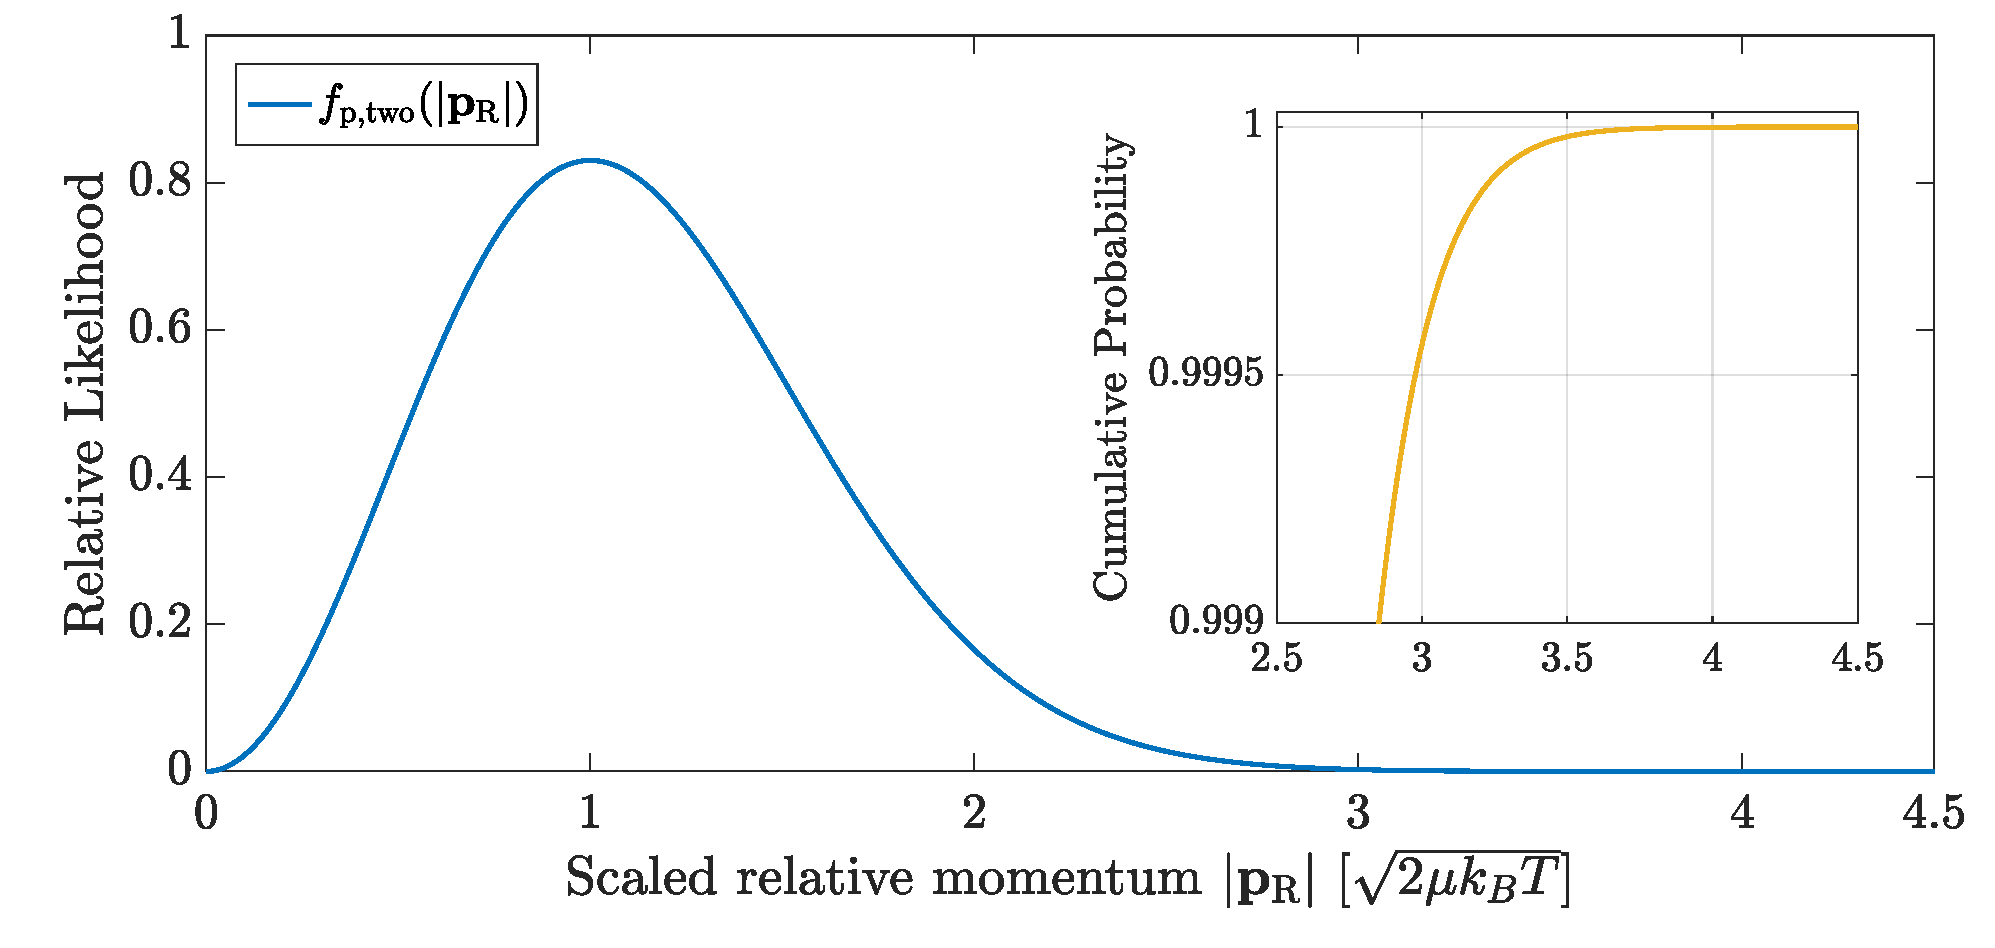
\includegraphics[width=\textwidth]{boltzmannFunc.pdf}}
		\caption{Two-particle Boltzmann distributions}{Equilibrium distributions of the momentum distribution Eq.\,\ref{eq:5mbmom} (blue) and the relative collision energy distribution \ref{eq:5mben}(red). Here $|\vec{p}|$ and $\epsilon$ are given in units of $\sqrt{2 \mu k_B T}$ to emphasize the generality of the distribution. Importantly, the likelihood of finding a particle with a momentum $|\vec{p}| > 4\sqrt{2 \mu k_B T}$ is extremely small. This is corroborated by the inset which shows the integral of the relative likelihood, also known as the cumulative distribution function of $f(|\vec{p}|)$. This gives the probability that a particle will take a value between $0 \rightarrow p_i$ for any specified $p_i$. Thus the probability for a particle to have momentum $|\vec{p}| < 4\sqrt{2 \mu k_B T}$ is $\approx\,1$.}
		\label{fig:singleBoltz}
	\end{figure}
We see that the occupation of momentum states $> 4\,\sqrt{2 \mu k_B T}$ is very small.
Therefore, in deep traps, when modeling photoassociation and calculating the scattering probability $\vert S(\epsilon) \vert^2$ over the relative collision energies, the unit probability remains conserved since nearly all possible collision energies are integrated over.
Conversely, a naive truncation of the Maxwell-Boltzmann integral when evaluating $\langle K \rangle_\text{thermal} \propto \displaystyle \int_0^{\epsilon_{max}} \vert S(\epsilon) \vert^2 d\epsilon$, will neglect the scattering probability of relative collision energy states above the integration limit $\epsilon_{max}$.
The likelihood of collisions at each relative energy is properly weighted by applying the energy cutoff to the single-particle kinetic energy distributions and then deriving the two-body relative energy distribution using the truncated forms of the single-particle distributions.
The modified form of the relative energy distribution will then be used in the thermal averaging of the two-body loss rate constant, $K$.

Before proceeding, we note that for descriptions of one-photon photoassociation with alkali atoms using dipole-allowed transitions, the consideration of single-particle kinetic energy may be neglected due to the natural width of the transition dominating any small shifts due to Doppler effect from center-of-mass motion or photon recoil.
For narrow-line one-photon PAS, Doppler shifts and photon recoil can become important due to the long-lifetime of the excited state \cite{Ciuryo2004, Borkowski2014a, Nicholson2015a, Reschovsky2018, Pachomov2017}.
Therefore, accurate enumeration of the scattering probability must consider and average over both the center-of-mass and relative kinetic energy distributions.
Our approach to the treatment of the truncation, outlined below, was informed and motivated by this common consideration for one-photon intercombination line PAS in strontium.
We emphasize that for these particular two-photon experiments, we are not sensitive to Doppler shifts or photon recoil.
%In
%
%however, the two-photon excitation process for these experiments being insensitive to Doppler shifts or photon recoil.

%For the experiments in this chapter, we are not sensitive to Doppler effects or photon recoil as the two-photon spectroscopy was performed with beams sharing a common wavevector.
%The previous work of Ref.\,\hl{\cite{Ciuryo2004, Borkowski2014a, Nicholson2015a, Reschovsky2018, Pachomov2017}} informed the approach taken here.
% is performed by integrating over both .
%the consideration of single-particle momenta and kinetic energies is commonly applied to the case of one-photon photoassociation performed near long-lived transitions where the narrow transition linewidth results in PAS that is sensitive to Doppler broadening and photon recoil \hl{\cite{Ciuryo2004, Borkowski2014a, Nicholson2015a, Reschovsky2018, Pachomov2017}}.


App.\,\ref{sec:truncDist} details the complete derivation of a normalized truncation function $\hat{\mathcal{G}}$, given by Eq.\,\ref{eq:truncWeighting}, which properly weights the possible collision energies.
With this weighting function, the distribution of relative energies is given in terms of dimensionless variables $\eta_\vec{r}$ and $\tilde{\epsilon}$ by
\begin{equation} \label{eq:truncRelBolz}
	\hat{f}_{\vec{r}}(\tilde{\epsilon}) = \frac{2}{\sqrt{\pi}} \sqrt{\tilde{\epsilon}} \, e^{-\tilde{\epsilon}} \hat{\mathcal{G}}(\eta_{\vec{r}}, \tilde{\epsilon})
\end{equation}
where
\begin{equation}
	\eta_\vec{r} = \frac{U_\text{depth} - U(\vec{r})}{k_B T} \quad \quad \tilde{\epsilon} = \frac{p_\text{R}^2}{2 \mu k_B T} 
\end{equation}
Here $\eta_\vec{r}$ is a scaled variable that defines the local maximum single-particle kinetic energy at a point $U(\vec{r})$ in the trap.
Similarly, $\tilde{\epsilon}$ gives the relative collision energy scaled by the temperature.
For each point in the trap, $\tilde{\epsilon}$ may take on the range of available energies $[ 0 \rightarrow 2\eta_\vec{r} ]$ where the upper bound on collision energy considers the case that both particles involved in the collision have kinetic energy $\displaystyle \frac{(U_\text{depth} - U(\vec{r}))}{k_B T}$.
The Heaviside function is used in $\hat{\mathcal{G}}(\eta_{\vec{r}}, \tilde{\epsilon})$ to ensure the collision energy cannot exceed $2\eta_\vec{r}$.

Fig.\,\ref{fig:relativeCollProb} plots the relative likelihood of collision energies for several values of $\eta_\text{trap}$.
	\begin{figure} 
	\centerline{
	  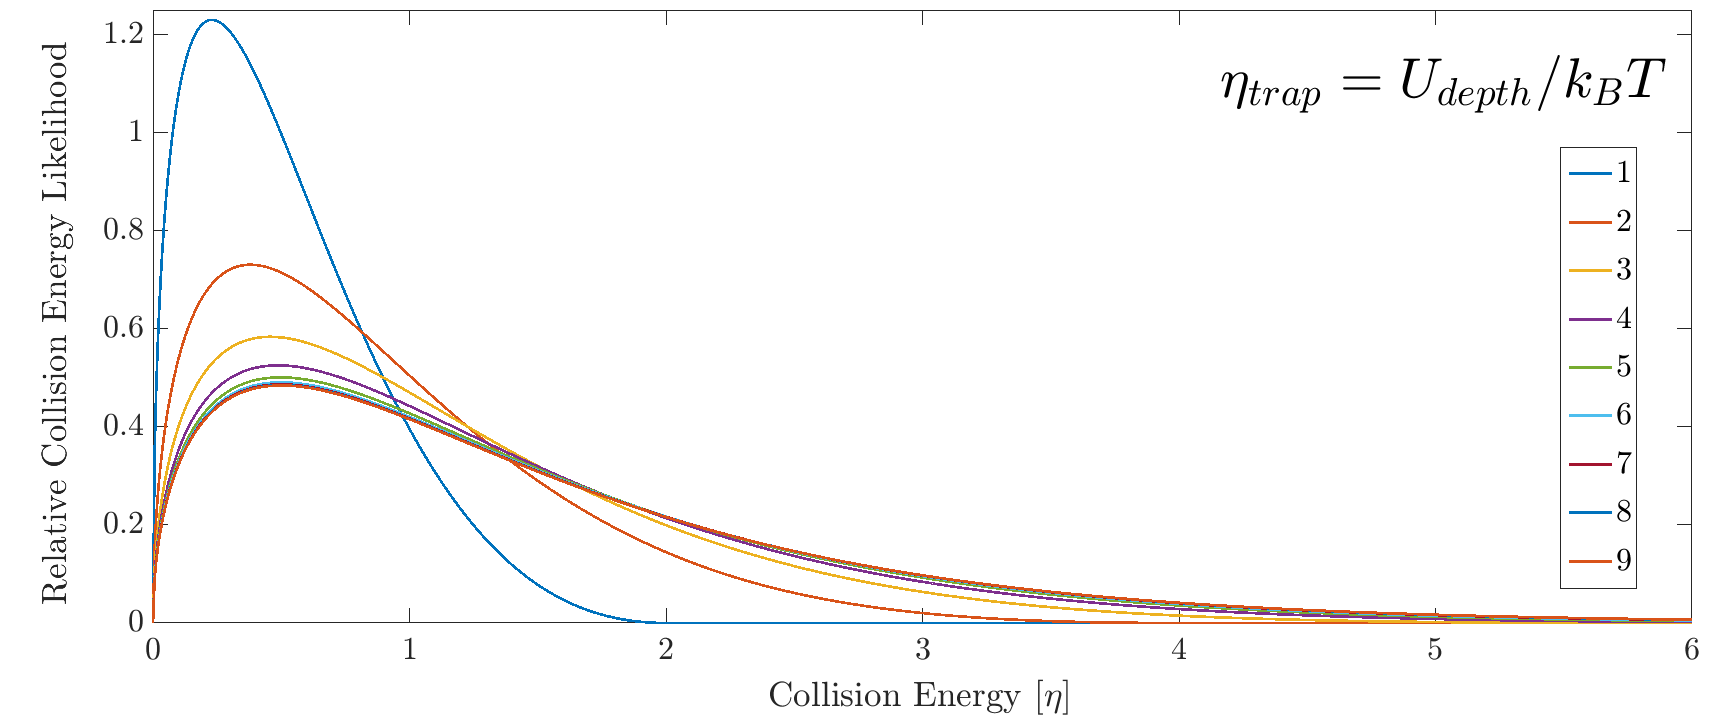
\includegraphics[width=\textwidth]{1DrelativeCollProbvsCollEn.png}}
	  \caption{Relative collision energy distributions for various trap depths}{The effects of energy truncation on the likelihood of collisions at different various trap depths where the total collision probability for each curve is normalized to unity. Energy is specified in units of $\eta = U_{\text{depth}}/k_B T$. Each trap has a maximum collision energy of $2\eta_{trap}$ between two particles each with maximum kinetic energy $\eta$.}
	  \label{fig:relativeCollProb}
	\end{figure}
In this plot, the collision energy is specified in units of $\eta$ such that $\eta=1=U_\text{depth}/k_B T$.
We see that for the case of $\eta_\text{trap}=1$ (blue curve), the maximum collision energy is $2\eta_\text{trap}$ and the likelihood falls to zero for higher energies as required by our definition of the truncation.
Furthermore, the relative energy distribution converges to a Maxwell-Boltzmann for trap depths $\eta_\text{trap} \gtrsim 4$.
This is in agreement with the expectations from the equilibrium distribution discussed at the beginning of this section.
Additional tests of the normalization and behavior of $\hat{\mathcal{G}}(\eta_{\vec{r}}, \tilde{\epsilon})$ are given with the derivation in the appendix.

\subsection{Fitting the thermally averaged spectra} \label{sec:lowIntSpectra}
The consideration of the relative collision energy likelihood is incorporated into the PAS lineshape equations by modifying the thermal average, $\langle K \rangle_\text{thermal}$.
Recall from Sec.\,\ref{sec:bohn_and_julienne}, that the two-body loss rate is simply given by $K= v \sigma_{in}$ and the thermal average is $\langle K \rangle_{\text{thermal}} = \int_0^{\infty} dv f(v)\,v\,\sigma_{in}$.
By replacing $f(v)$ with Eq.\,\ref{eq:truncRelBolz} and modifying the integration bounds, the truncated thermal average may be given by
\begin{equation}
	\langle K \rangle_\text{thermal} = \frac{1}{h\,Q_{T}} \int_{0}^{2\,\eta} d\epsilon \vert S(\epsilon) \vert^2 \, \hat{\mathcal{G}}(\eta, \tilde{\epsilon})\,\exp{\frac{-\epsilon}{k_{B}T}}
\end{equation}
where $\tilde{\epsilon} = \epsilon/k_{B}T$ and $\eta$ is the single-particle truncation energy.
This integral is limited to $\epsilon = 2\,\eta$ to account for both particles having the maximum energy $\eta$ while undergoing a collision.
Note that, while this discussion began by considering the effects of shallow traps, the above expression only concerns the energetic portion of the problem.
The complete two-body loss rate with averages over collision energy and space and incorporating the effects of local collision energy truncation becomes
\begin{align} \label{eq:chap5avgTruncK}
\hspace*{-1cm} 
	\langle K \rangle_\text{trunc, trap} = \frac{1}{V_2} \int_V &\exp{\frac{-2 U(\vec{r})}{k_{B}T}} \\ 
	\nonumber
	&\times \frac{1}{h\,Q_{T}} \int_{0}^{2\,U_{\text{depth}}(\vec{r})} d\epsilon \vert S(\epsilon, \vec{r}) \vert^2 \,\hat{\mathcal{G}} \left[\frac{U_\text{depth}-U(\vec{r})}{k_B T}, \frac{\epsilon}{k_{B}T}  \right]  \,\exp{\frac{-\epsilon}{k_{B}T}}
\end{align}
where $U_\text{depth}$ is a global parameter describing the trap depth and we have explicitly stated the inputs to the function $\hat{\mathcal{G}}(\eta_{\vec{r}}, \tilde{\epsilon})$.

However, due to the geometry of the trap, as discussed above, $U_\text{depth}$ is not a clearly defined quantity.
Fig.\,\ref{fig:truncatedSpectraFit}a shows lineshape fits for several different values of the trap depth applied to the same spectrum.
	\begin{figure}
	\centerline{
	  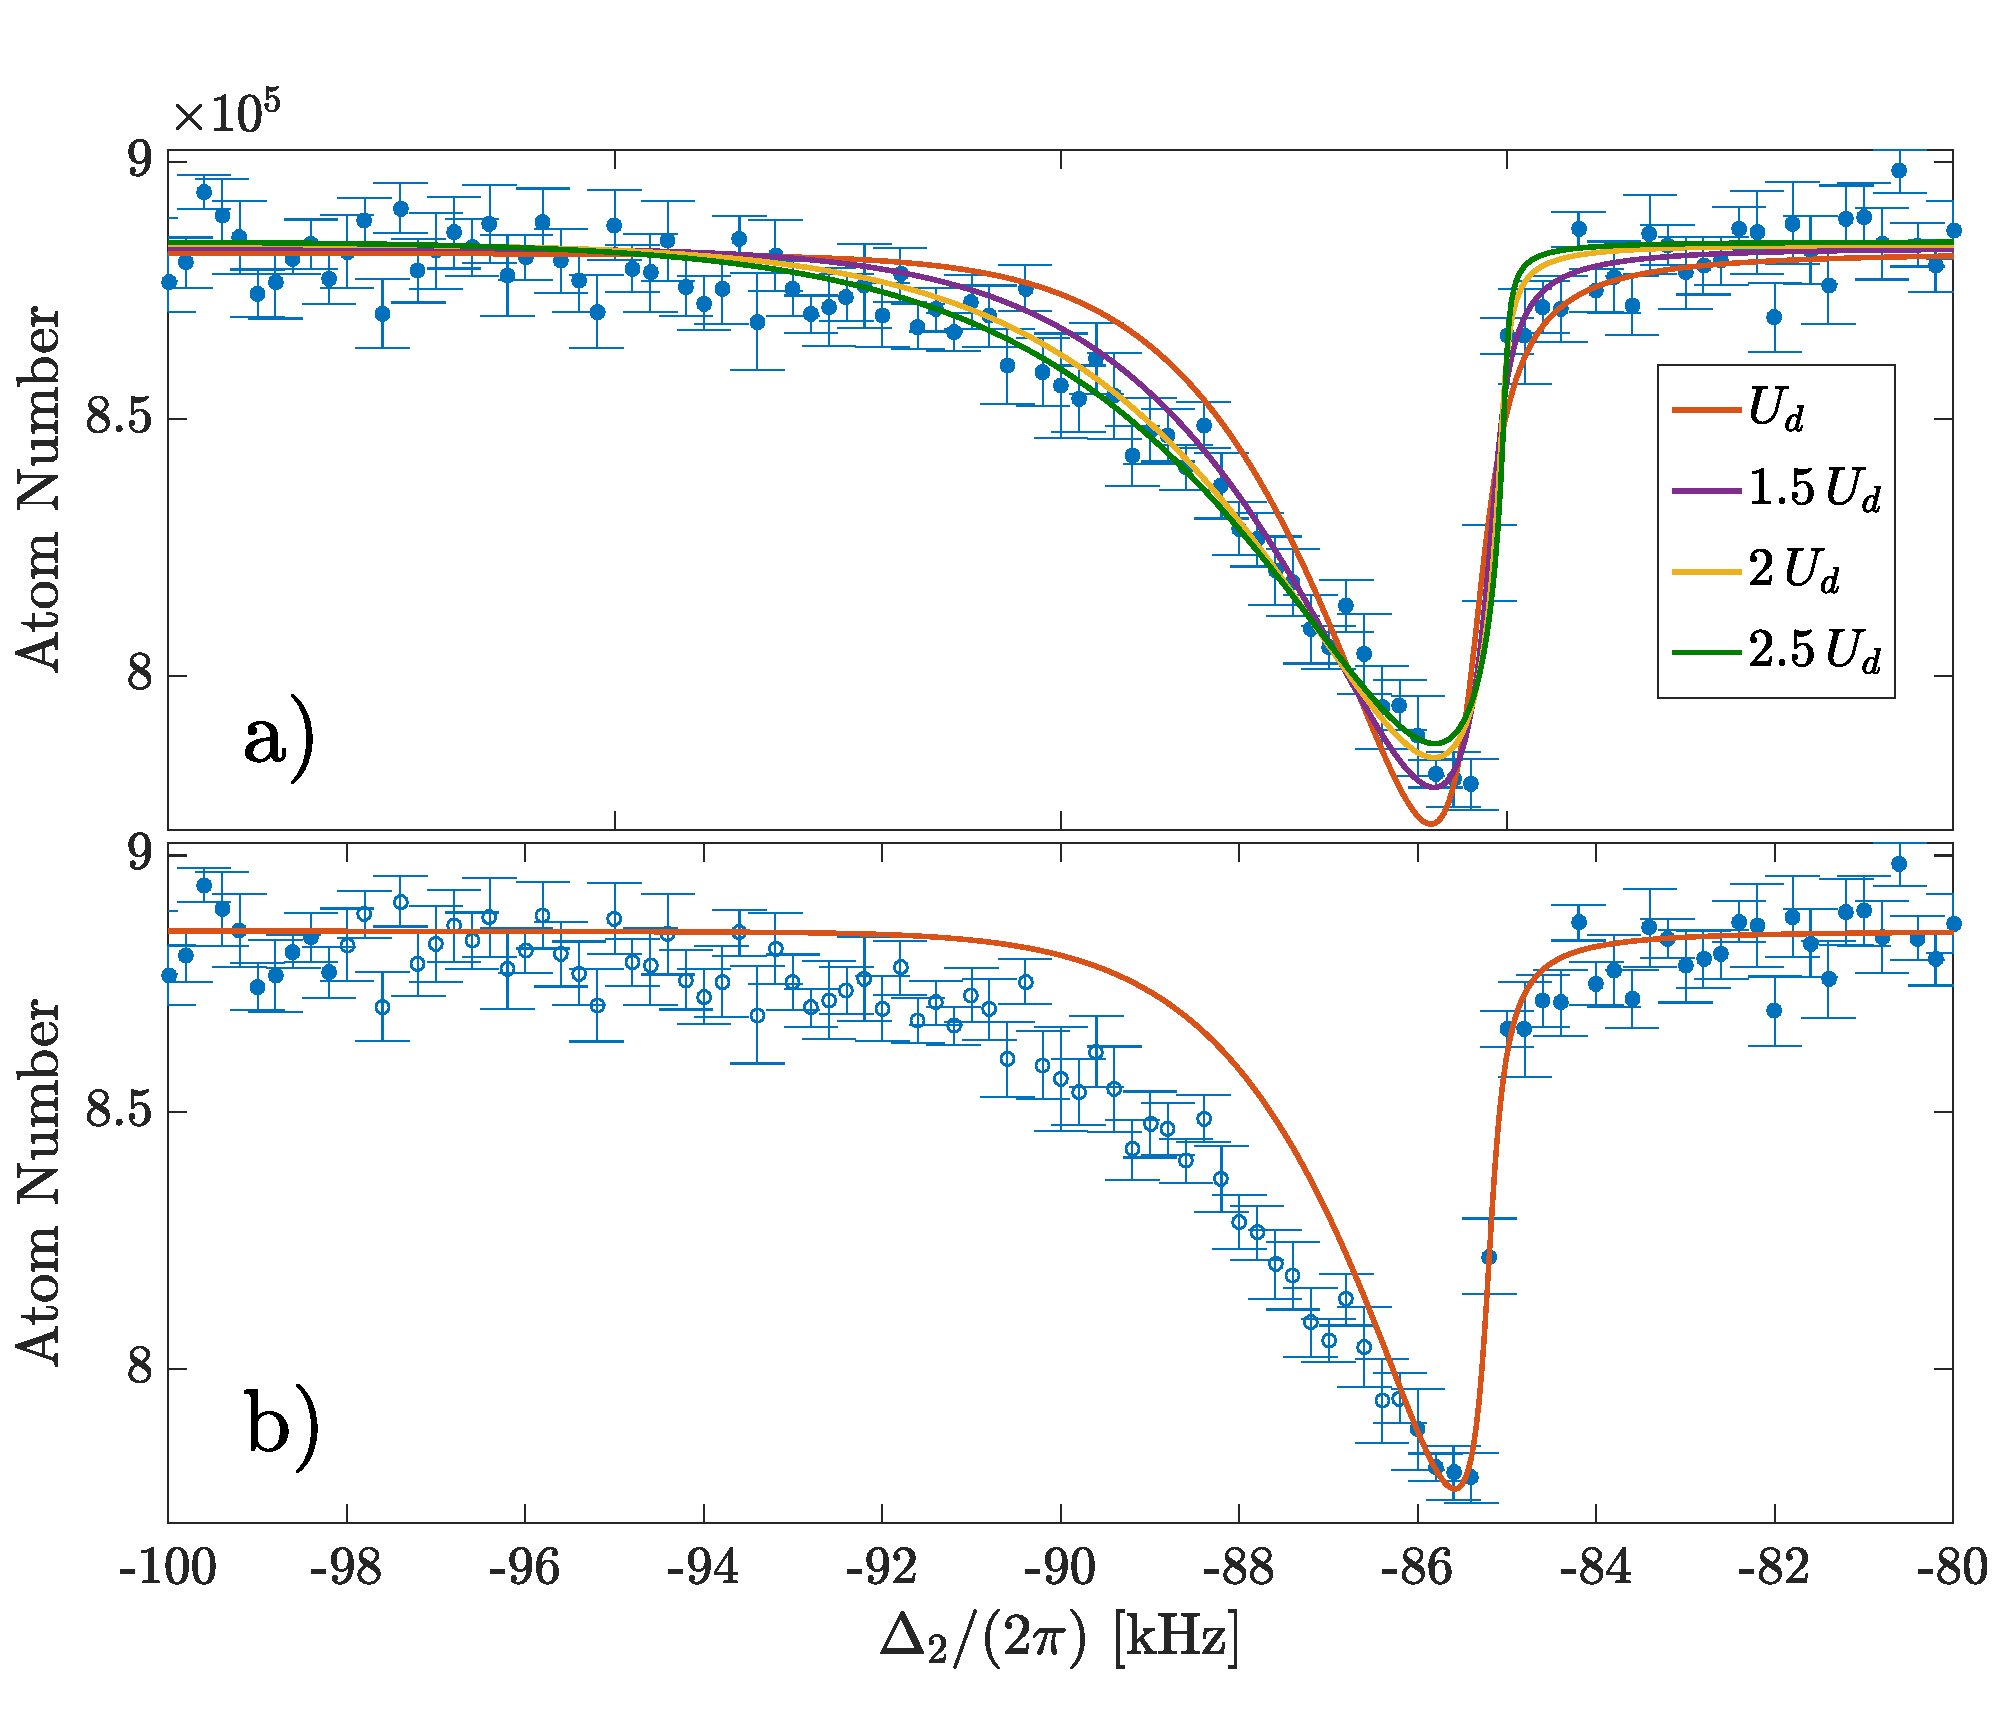
\includegraphics[width=\textwidth]{truncated_fixU_compare.pdf}}
	  \caption{Comparison of lineshape fits at various $\epsilon_{\text{max}}$}{Using a constant trap geometry (eg. Fig.\,\ref{fig:haloTrapModel}) with a trap depth $U_d$. Sample temperature determined from time-of-flight is 100\,nK. a) The spectrum is fit with varying maximum collision energy, $\epsilon_{\text{max}}$. The solid lines are labeled by the trap depth which is the maximum single particle kinetic energy. b) The spectrum is fit, neglecting the effects of truncation, using only the filled data points.}
	  \label{fig:truncatedSpectraFit}
	\end{figure}
Here we can clearly distinguish the behavior of the fitting algorithm.
Starting with the trap depth at $U_\text{depth}$ (red curve), the model cannot account for the large energy distribution in the tail so the effective width $\gamma_{\text{eff}}$, is increased by the algorithm resulting in a fit that does not accurately capture the binding energy, the thermal tail, or the sharp edge of the lowest energy collisions.
As the single-particle energy is increased, the width decreases and begins to capture the thermal distribution as well as the sharp edge.
To estimate the systematic uncertainty introduced by this treatment, we perform fits with $\epsilon_{\text{max}}$ equal to $2[U_{\text{depth}}-U(\mathbf{r})]$ and $U_{\text{depth}}-U(\mathbf{r})$ and take the mean of the two results as the best value for the binding energy and half the difference as a systematic uncertainty $\sigma_{\epsilon_{\text{max}}}\approx 100$\,Hz.
This procedure does not correctly represent the overall normalization of $\vert S \vert^2$, but we are not concerned with overall signal amplitude in this study.

Alternatively, as the molecular binding energy is strongly determined by the sharp edge of the spectrum that is relatively insensitive to the description of the broad red tail, we exclude the thermal portion and fit just the edge, neglecting any effects of truncation.
An example of such a fit is shown in Fig.\,\ref{fig:truncatedSpectraFit}b.
The resulting estimates of the binding energies from both analyses agree within error.
Using only the values from the edge fit method does not substantively change our conclusions in the following sections.

\section{Determination of energy shifts} \label{sec:lowE_Eb2}
We estimate the halo resonance energy with fits of the atom-loss spectra using Eq.\,\ref{eq:number} for the evolution of atom number with time, Eq.\,\ref{eq:chap5avgTruncK} for the average two-body loss rate constant over the trap volume and locally truncated collision energy, and the phenomenological expression Eq.\,\ref{5equationApproxLorentzian} for the scattering probability.
The shifted resonance energy $E'_{b2}$, $\eta$, and $\gamma_{\text{eff}}$ are taken as fit parameters. 
In the final analysis, temperatures are set to values determined from time-of-flight imaging of the atoms, but when they are allowed to vary, the fit values differ by no more than 10\%.
Approximately 10 spectra are recorded and independently fit for each set of experimental parameters.
The spread of resulting parameter estimates from the fits are used to determine best values and uncertainties.
All error bars shown are the standard error determined from the set of individual scans.

The susceptibilities, in Hz per unit intensity or density, are determined from experimental data or theoretical considerations.
We take $I_{689}$ as twice the single-beam intensity $I_{689}=2I$ and the functional form for the AC Stark shift due to the excitation lasers as discussed in Sec.\,\ref{sec:highE_theory}.

\subsection{AC Stark shift due to excitation lasers}
The most significant perturbation to the resonance position is the AC Stark shift due to the excitation laser intensity, as shown in Fig.\,\ref{fig:SpectraVarying689Intensity}.
	\begin{figure} 
	\centerline{
	  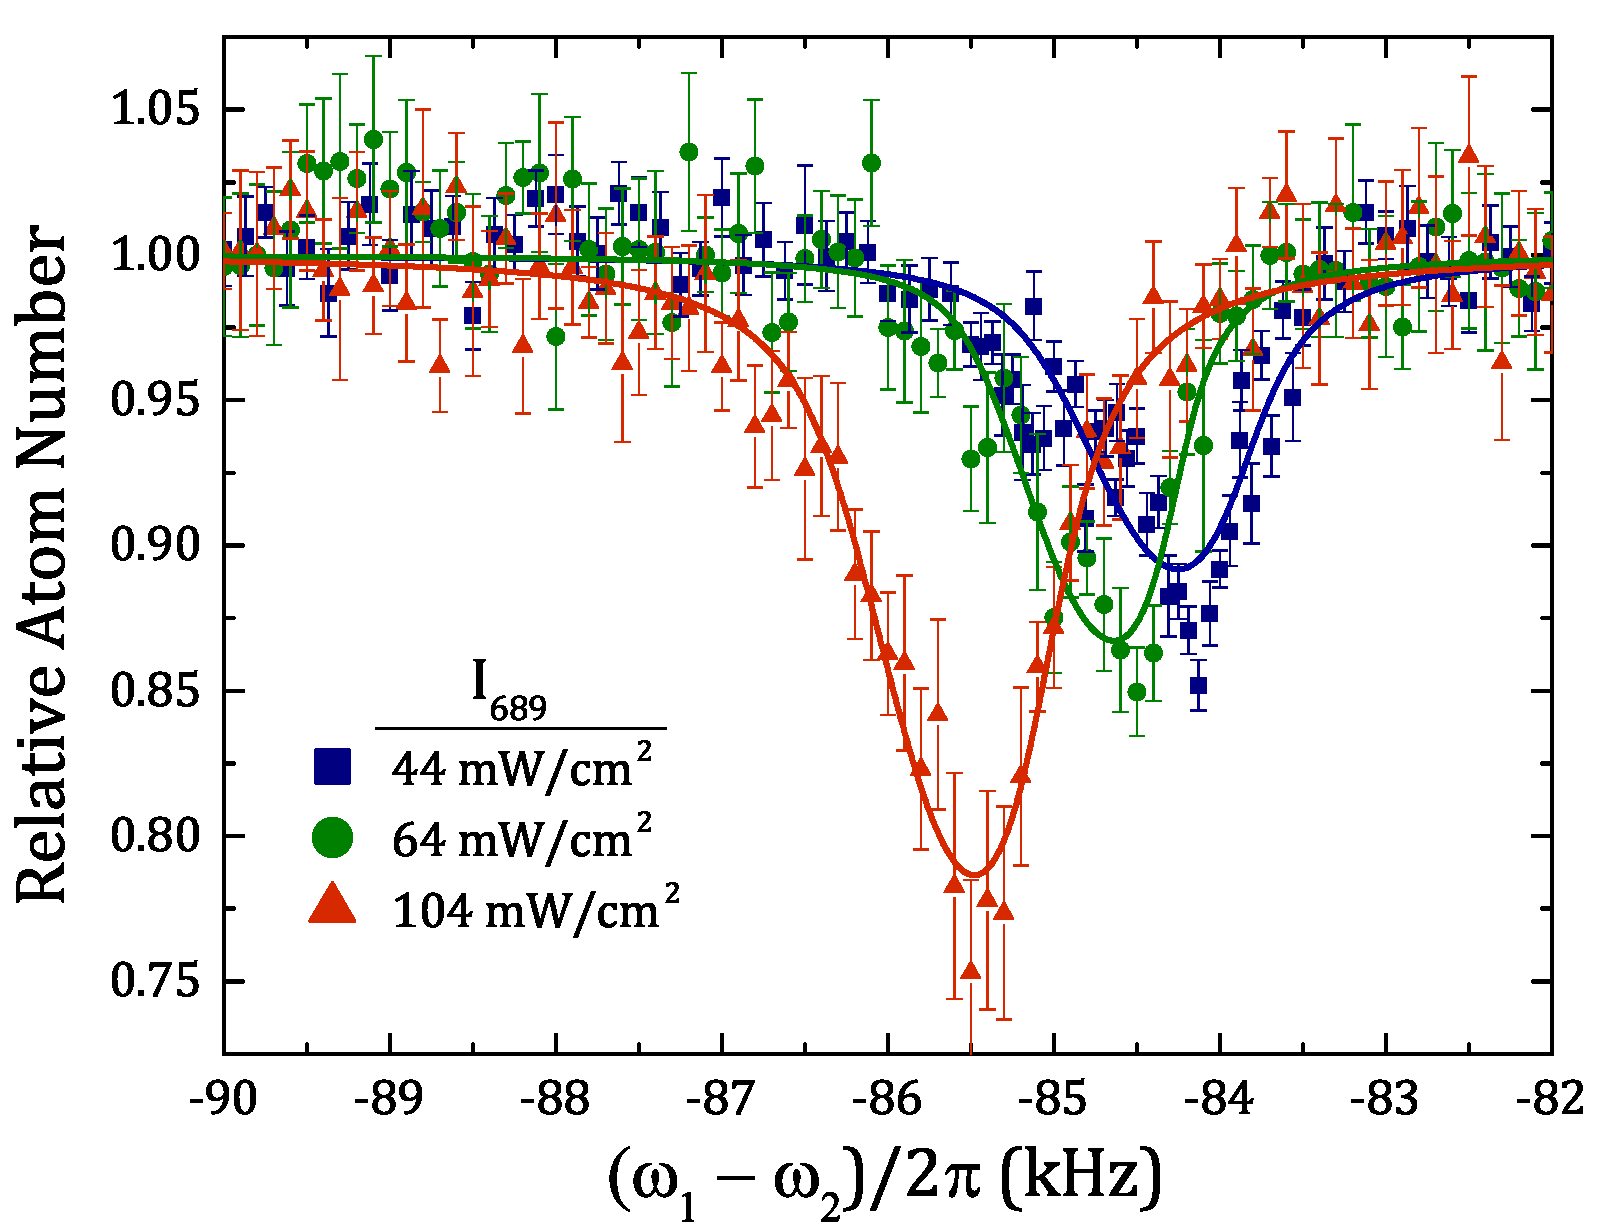
\includegraphics[width=\textwidth]{spectra_vary_689.pdf}}
	  \caption{Atom-loss spectra with varying $689$\,nm intensity}{Atom-loss spectra as a function of two-photon difference frequency $(\omega_1-\omega_2)/2\pi$ for intermediate detuning $\Delta_1/2\pi=-9$\,MHz and various $689$\,nm excitation laser intensities. Twice the single-beam intensity $I_{689}=2I$ is indicated in the legend.}
	  \label{fig:SpectraVarying689Intensity}
	\end{figure}
When this data is fit using the methodology described above (with two different values for $U_\text{depth}$) the estimate of the binding energy is consistent and the model lineshapes do not differ substantially.
Therefore, only the model with trap depth $U_\text{depth}$ is shown.
	
For this data, the trap parameters, temperature ($T=30$\,nK), and initial peak sample density ($n_0=2\times 10^{12}$\,cm$^{-3}$) are held constant.
We varied the single-beam excitation intensity from $I=0.02-0.06$\,mW/cm$^{-2}$, and the excitation time was 50\,ms.
The observed shifts are comparable to the thermal width of the spectrum, allowing a precise determination of $\chi_{689}=-21(1)(2)$\,kHz/(W/cm$^{2})$ from a linear fit to the resonance positions, $E'_{b2}\propto h\chi_{689} I_{689}$ as shown in Fig.\,\ref{fig:ShiftWith689Intensity}).
	\begin{figure}
	\centerline{
	  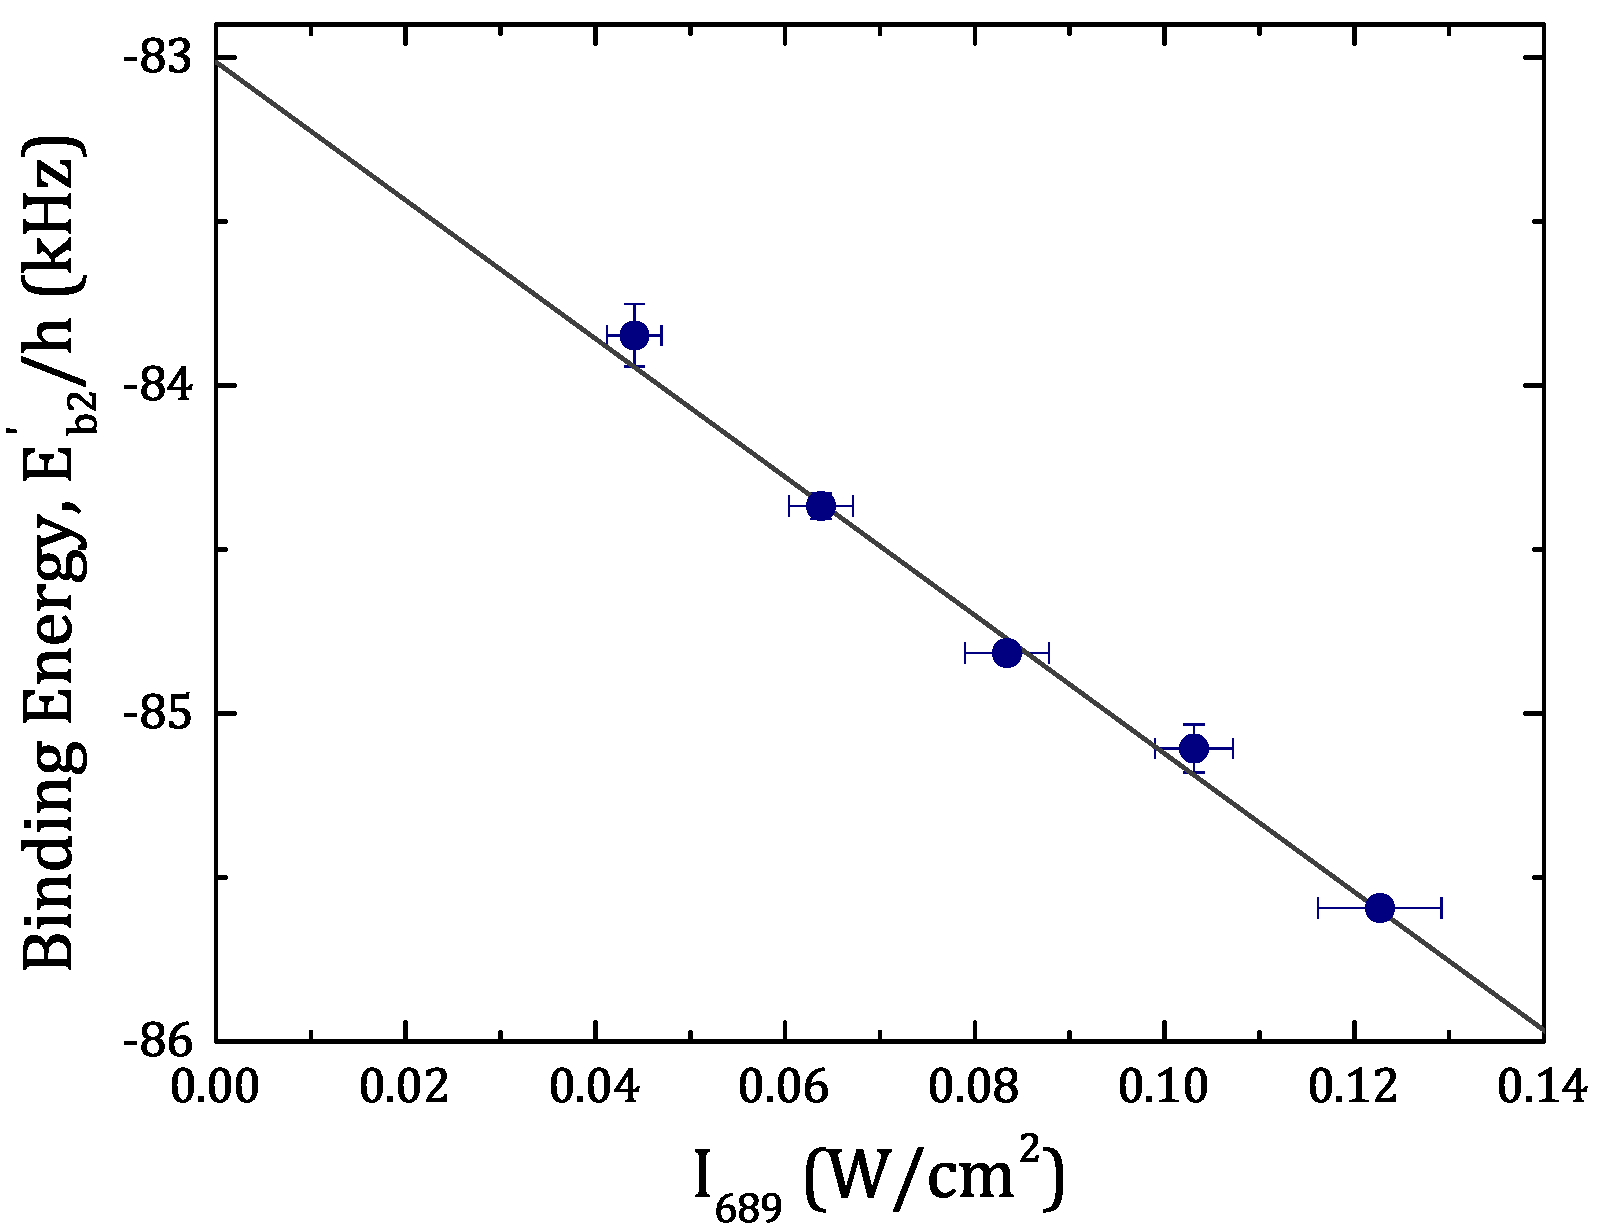
\includegraphics[width=\textwidth]{halo_susceptibility_689.pdf}}
	  \caption{Fit of $689$\,nm AC Stark shift}{Measured resonance position $E_{b2}'$ plotted versus twice the single-beam intensity $I_{689}=2I$ . The linear fit provides the AC Stark shift parameter $\chi_{689}$.}
	  \label{fig:ShiftWith689Intensity}
	\end{figure}
The first quoted uncertainty is statistical and it arises from variations in parameters and fluctuations in the measured intensity during the scans.
The second value is systematic, reflecting uncertainty in laser-beam size and intensity profile at the atoms.
This is comparable to the estimate of the Floquet model that was developed using the high-intensity data.

All parameters beside the $689$\,nm laser intensity are held fixed for this data, and the AC Stark shift is not correlated with any other variable, such as density or trap intensity.
We thus obtain an accurate measure of $\chi_{689}$ without attempting to account for other systematic shifts of $E'_{b2}$ in this data.

Broadening to the blue side of the spectrum is most sensitive to decay of the intermediate state $\Gamma_L(\epsilon)$, and the additional broadening term $\gamma_{\text{eff}}$. 
The long lifetime of the excited state and the significant detuning $\Delta_1$ result in a width $\Gamma_L(\epsilon) < 5\,\text{Hz}$ for all conditions.
This is extremely small compared to the observed width, which estimates $\gamma_{\text{eff}}$ on the order of $300\,\text{Hz}$.
We hypothesize that this width reflects decay of molecules in the electronic ground-state due to collisions with background atoms.

\subsection{Density-dependent frequency shift}
A shift of the two-photon resonance position is possible due to differing mean-field shifts of initial atomic and final molecular states arising from interaction with the background of ground-state atoms.
Such a shift would be proportional to the atom density and depend upon the $s$-wave scattering lengths for atom-atom and atom-dimer collisions, $a_{86}$ and $a_{\text{ad}}$ respectively.
This was observed in a Rb Bose-Einstein condensate in Ref.\,\cite{wfh00}. 
For a non-degenerate gas, this effect yields $\chi_n=\hbar (\frac{a_{\text{ad}}}{\mu_{\text{ad}}}-4\frac{a_{86}}{\mu_{\text{aa}}})=\frac{\hbar}{m} (\frac{3 }{2}a_{\text{ad}}-8 a_{86})$, where $\mu_{\text{ad}}$ and $\mu_{\text{aa}}$ are the reduced masses for molecule-atom and atom-atom collisions respectively.
Note that the shift would vanish for $a_{\text{ad}}=(16/3) a_{86}$.
The largest densities used in these experiments was $\sim 1-2\times 10^{12}\,\mathrm{cm}^{-3}$.
This is relatively low compared to typical BEC densities, and at this time we are unable to accurately measure a variation of resonance position with density.
However, the atom-atom scattering is close to resonance and thus Efimov physics can provide information on $a_{\text{ad}}$ \cite{bha07,nen17} and an estimate of the systematic error introduced by any residual density-dependent frequency shifts.
For a zero-range interaction, the atom-dimer scattering length is related to the atom-atom scattering length through the three-body Efimov parameter $\kappa_*$ according to \cite{bha07}
\begin{equation}\label{Eq:EfimovMoleculAtomScatteringLength}
  a_{\text{ad}}=a_{86}\left\{1.46 + 2.15 \mathrm{cot}[s_0 \mathrm{ln} (14.1\kappa_* a_{86}) ]\right\}
\end{equation}
where $s_0=1.006$ \footnote{The Efimov parameter is related to $E^0_{3b}$ through $\kappa_*=(m|E^0_{3b}|/\hbar^2)^{1/2}$, where $E^0_{3b}$ is the binding energy the lowest Efimov trimer would have in the case of resonant atom-atom interactions.}.

In principle, the atom-dimer scattering length can take any value.
However, for a deep atom-atom potential, such as for the ground-state strontium dimer \cite{Stein2010}, there is a universality of the three-body physics that sets $\kappa_*=0.226(2)/R_{\mathrm{vdW}}$ \cite{wie12}.
Here, $R_{\mathrm{vdW}}=\left({2\mu C_6}/{\hbar^2}\right)^{1/4}/2=74.6$\,$a_0$ is the van der Waals length associated with the $C_6$ coefficient of the long-range Sr$_2$ ground-state potential.
Using $C_6=3164$a.u.\;from a fit of potential parameters to spectroscopic data \cite{Stein2010}, yields $\kappa_*=5.72\times 10^7$\,m$^{-1}=(330\,a_0)^{-1}$.
Eq.\,\ref{Eq:EfimovMoleculAtomScatteringLength} then predicts $a_{\text{ad}}=6.4\, a_{86}$, which leads to a small density-dependent frequency shift parameter of $\chi_n=50\,\mathrm{Hz}/(10^{12}\,\mathrm{cm}^{-3})$.
A numerical calculation including a finite-range correction for the atom-atom interaction \cite{mwc17} results in $a_{\text{ad}}=3.5\, a_{86}$ and $\chi_n=-90\,\mathrm{Hz}/(10^{12}\,\mathrm{cm}^{-3})$.
Thus, a very small shift is expected for the densities used here.

We incorporate $\chi_n=0\pm 90 \,\mathrm{Hz}/(10^{12}\,\mathrm{cm}^{-3})$ as a set parameter in our model of the spectrum, where we set the systematic uncertainty to reflect the spread of theory predictions.
This uncertainty is the most significant source of error for our determination of the unperturbed halo binding energy.

\subsection{AC Stark Shift due to Trapping Lasers}
Fig.\,\ref{fig:Spectraminus9MHzVaryTrapCold} shows a series of spectra for different final trap depths and sample temperatures.
	\begin{figure}
	 \centerline{
	 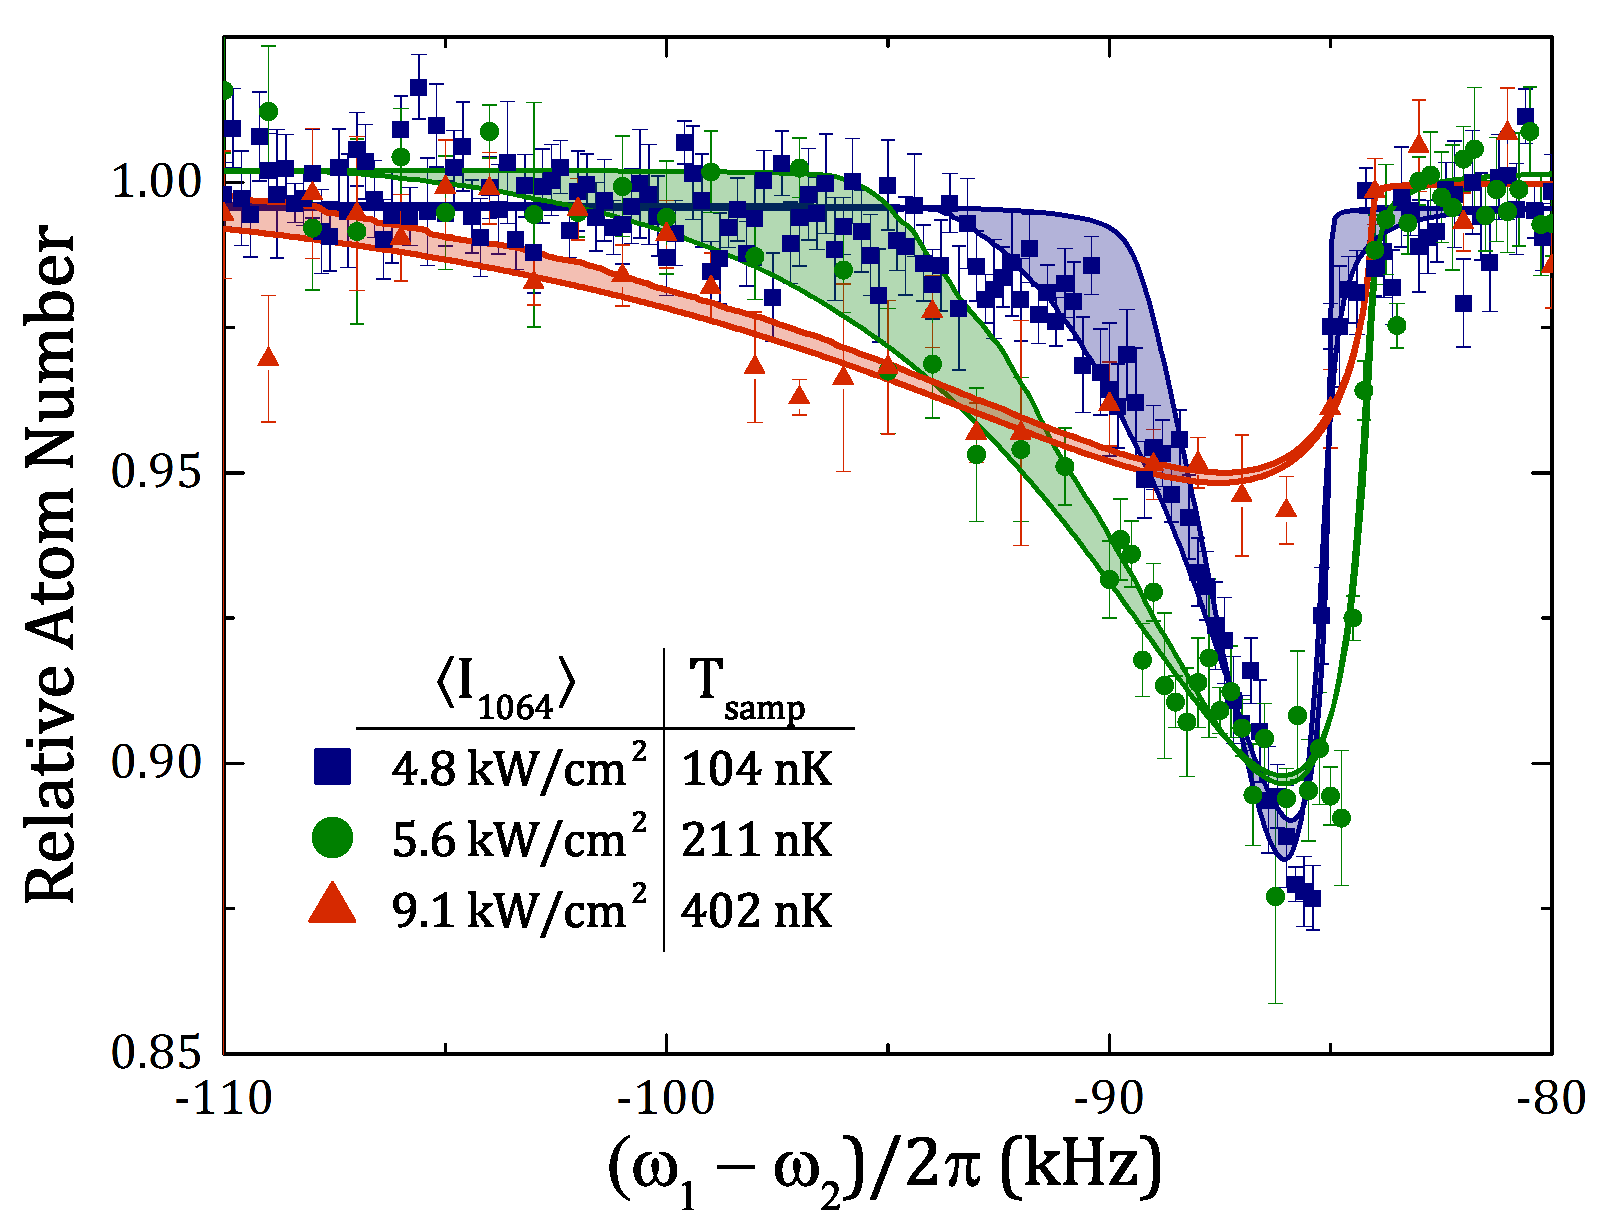
\includegraphics[width=\textwidth]{spectra_vary_1064.pdf}}
  \caption{Atom-loss spectra with varying $1064$\,nm intensity}{Sample temperature and average trapping laser intensity are indicated in the legend. The single-beam excitation laser intensity is $I=25$\,mW/cm$^{2}$ for the 104\,nK spectrum and $I=48$\,mW/cm$^{2}$ for the 211\,nK and 402\,nK spectra. The two boundaries of each band give the fits with collision-energy truncation
$\epsilon_{\text{max}}$ equal to $2[U_{\text{depth}}-U(\mathbf{r})]$ and $U_{\text{depth}}-U(\mathbf{r})$.}
  	\label{fig:Spectraminus9MHzVaryTrapCold}
	\end{figure}
Here the role of the truncation discussed in Sec.\,\ref{sec:trunc_trap} is noticeably more evident.
We illustrate this difference by bounding each fit with a solid line and shading the region between.

The final effect we considered accounts for spatial dependence of the AC Stark shift due to the intensity $I(\vec{r})$ of the $1064$\,nm trapping laser.
Models including this effect were used to fit the spectra and found no significant effects on the fitted parameter estimates within our knowledge of the trapping potential.
Therefore, as inclusion of this effect significantly increases the computation time of the lineshape, we approximated its effect by calculating a two-body weighted average intensity of the $1064$\,nm laser to characterize the average shift experienced by the atoms due to the trapping potential.

With an accurate determination of $\chi_{689}$, a value for $\chi_n$, and a method for characterizing the trapping intensity, we use the data shown in Fig.\,\ref{fig:Spectraminus9MHzVaryTrapCold} to determine the susceptibility for the AC Stark shift from the trapping laser, $\chi_{1064}$, and the unperturbed halo binding energy $E_{b2}$.
Fig.\,\ref{fig:ShiftWithTrapIntensity} shows a plot of $E_{b2}'-\chi_{689}I_{689} - \chi_{\text{n}}\langle n\rangle$ versus $\langle I_{1064} \rangle $, where $E_{b2}'$ is the resonance position from each fit and $\langle ... \rangle $ indicates a weighted average of the quantity over the trapped sample, with a weighting given by the square of atom density.
The plotted uncertainties in $E_{b2}'-\chi_{689}I_{689} - \chi_{\text{n}}\langle n\rangle$ are from statistical variation in the fit parameters.
	\begin{figure} 
	\centerline{
	  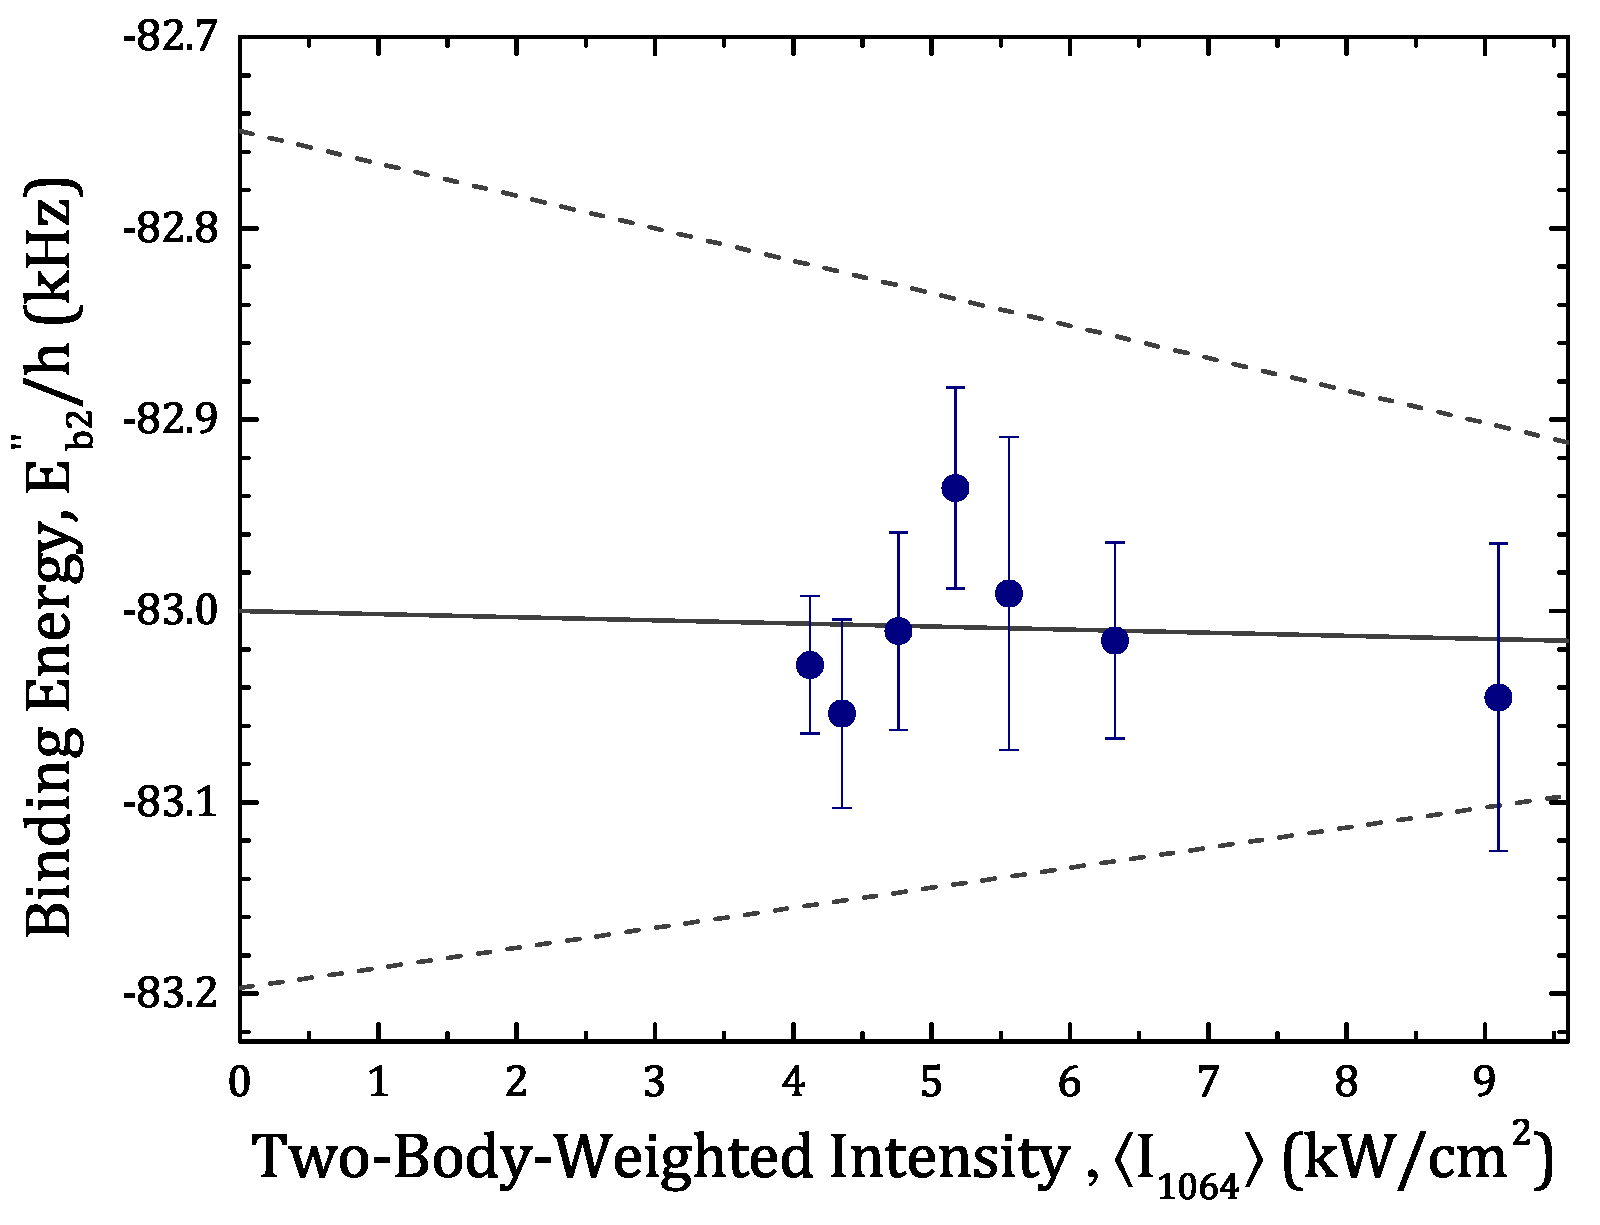
\includegraphics[width=\textwidth]{halo_susceptibility_1064.pdf}}
	  \caption{Measurement of halo state susceptibility, $\chi_{1064}$}{Measured resonance positions corrected for excitation-laser AC Stark shift and collisional frequency shift, $E_{b2}'-\chi_{689} I_{689} - \chi_{n}\langle n\rangle$, as a function of average trap laser intensity $\langle I_{1064} \rangle$ for the data such as in Fig. \ref{fig:Spectraminus9MHzVaryTrapCold} . The trend line and confidence intervals are described in the text.}
	  \label{fig:ShiftWithTrapIntensity}
	\end{figure}

The typical average density is $\langle n\rangle\approx 1\times 10^{12}$\,cm$^{-3}$. 
The linear fit function is to $E_{b2}+\chi_{1064}\langle I_{1064} \rangle $.
In addition to statistical uncertainty, we account for the systematic uncertainty from $\chi_{\text{n}}$ and our treatment of the truncation of the collision-energy integral by using the limiting estimates for each parameter in determining $E_{b2} = E_{b2}'-\chi_{689}I_{689} - \chi_{\text{n}}\langle n\rangle$ and performing a linear fit.
The dashed lines shown in Fig.\,\ref{fig:ShiftWithTrapIntensity} show the results of these fits.
The resulting value for the unperturbed binding energy is $E_{b2}/h=-83.00(7)(20)$\,kHz, where the first uncertainty is statistical, and the second is systematic.
We estimate a susceptibility to $I_{1064}$ of $\chi_{1064}=0\pm 10$\,Hz/(kW/cm$^2$).

\section{Discussion of the halo binding energy} \label{sec:lowE_alt}
In the limit of extremely small binding energy and resonant atom-atom interactions, the binding energy of a halo molecule is approximately given by \cite{Kohler2006, hle57, Chin2010}
\begin{equation} \label{Eq:HaloEnergyNoCorrections}
	E_b=\frac{\hbar^2/}{2\mu a^2}
\end{equation}
For interactions described at long-range by a van der Waals potential $V(r)=-C_6/r^6$, as with ultracold atoms, a convenient figure of merit for quantifying how accurate Eq.\,\ref{Eq:HaloEnergyNoCorrections} should be is given by the ratio of the $s$-wave scattering length to the interaction range $\bar{a}$ that is closely related to the van der Waals length \cite{gfl93,cju05}.
\begin{equation} \label{Eq:InteractionRangevdW}
  \bar{a} = \frac{4 \pi}{\Gamma(1/4)^2}R_\mathrm{vdW}
\end{equation}
Slightly away from resonance, corrections to the binding energy for the van der Waals potential were worked out in \cite{Gao01,gao04}, yielding
\begin{equation} \label{Eq:BindingEnergyGao}
	E_{b2}=-\frac{\hbar^2}{2\mu(a-\bar{a})^2}\left[1+\frac{g_1\bar{a}}{a-\bar{a}}+\frac{g_2\bar{a}^2}{(a-\bar{a})^2} + ... \right],
\end{equation}
where $g_1=\Gamma(1/4)^4/6\pi^2-2=0.918...$ and $g_2=(5/4)g_1^2-2=-0.947...$. 
The range of validity of this expression is $a \gtrsim 2 \bar{a}$.
The accuracy of the first term in this expansion has been experimentally confirmed for various systems such as $^{85}$Rb \cite{ckt03,kgb03}, $^{40}$K \cite{rtb03,msg05} and $^{6}$Li \cite{bar05}.
The derivation of Eq.\,\ref{Eq:BindingEnergyGao} assumes that the influence of short-range physics, which can be expressed through a quantum defect, varies negligibly from threshold to the molecular binding energy.
We expect this to be an excellent approximation, since, as shown in Ref.\,\cite{Gao01} the corrections are typically less than about $1\%$ even for GHz binding energies.

For ground-state $^{86}$Sr atoms, $\bar{a}=71.3$\,$a_0$.
The most accurate value available for the $s$-wave scattering length is $a=798 (12)$\,$a_0$ \cite{Stein2010}, satisfying the requirement of $a\gg \bar{a}$ for the least-bound state on the ground molecular potential to be a halo molecule.
Nonetheless, ${\bar{a}}/({a-\bar{a}})=.10$, and the corrections given by Eq.\,\ref{Eq:BindingEnergyGao} are seen to be significant in Fig.\,\ref{fig:HaloBindingEnergy}.
	\begin{figure} 
	\centerline{
	  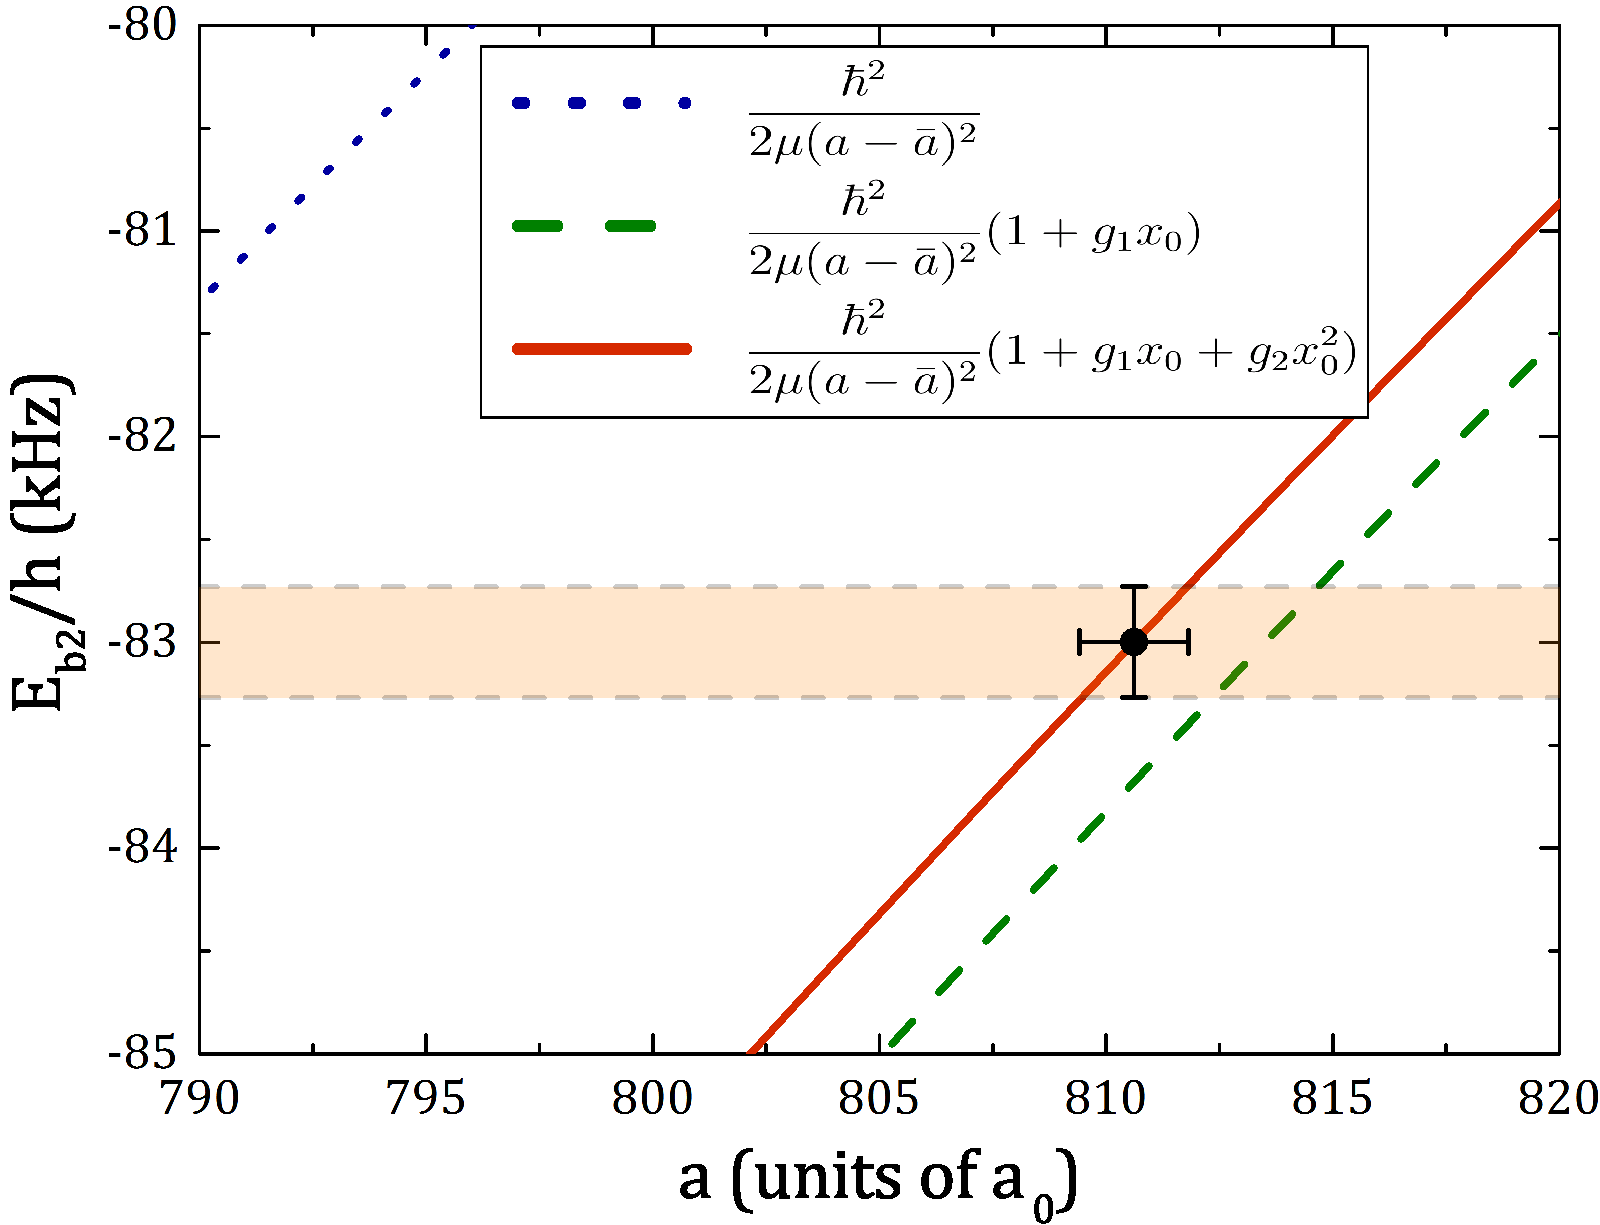
\includegraphics[width=\textwidth]{86_scattering_length.pdf}}
	  \caption{Determination of 86 $s$-wave scattering length}{Halo binding energy versus $s$-wave atom-atom scattering length for $^{86}$Sr . The shaded region indicates our experimental measurement. The lines are predictions of Eq.\,\ref{Eq:BindingEnergyGao} retaining up to the first, second, and third terms as indicated in the legend [$x_0={\bar{a}}/({a-\bar{a}})$]. The data point is the prediction of Eq.\,\ref{Eq:BindingEnergyGao} for the recommended value of the measured binding energy.}
	  \label{fig:HaloBindingEnergy}
	\end{figure}
Using the previous best value of the scattering length, Eq.\,\ref{Eq:BindingEnergyGao} predicts a binding energy of $E_{b2}=-86(3)$\,kHz.
This agrees with our measurement, but by inverting Eq.\,\ref{Eq:BindingEnergyGao}, we can use our increased accuracy in $E_{b2}$ to extract an improved value of the scattering length of $a=810.6(3)(9)$\,$a_0$, where uncertainties reflect statistical and systematic uncertainties in $E_{b2}$ respectively.
The next higher-order term in $x_0={\bar{a}}/({a-\bar{a}})$ is likely to introduce a correction on the order of $100$\,Hz in Eq.\,\ref{Eq:BindingEnergyGao}, creating a systematic uncertainty in $a$ that is about one third of the uncertainty from our measurement.

This binding energy can also be used to estimate the value of the ground state potential $C_6$ parameter for strontium.
As previously discussed in Sec.\,\ref{ssec:low_energy}, the relationship between the scattering length and the potential is given by
\begin{equation} \label{eq:5scatterLeng}
	a = \bar{a} \left[ 1 - \tan(\Phi - \frac{\pi}{8}) \right] \quad \quad \Phi = \int_{R_i}^{\infty} dR \sqrt{\frac{-2\mu V(R)}{\hbar^2}}
\end{equation} 
where $R_i$ is the inner turning point of the potential such that $V(R_i)=0$.
Therefore, given the potential, we can use these equations to calculate the $s$-wave scattering length and then use Eq.\,\ref{Eq:BindingEnergyGao} to estimate the binding energy of the halo state.

Stein et al. (2010) \cite{Stein2010}, gives two piece-wise estimates of the strontium ground state X$^1\Sigma_g^+$ potential determined from molecular spectroscopy data.
The two model potentials are labeled "freely varied" and "recommended".
Each model is derived from estimating long-range coefficients by fitting the transition data and subsequently comparing to $\textit{ab initio}$ calculations.
The "freely varied" model results from allowing all long-range coefficients to be treated as fit parameters and subsequently estimated by the fitting routine routine.
The "recommended" model is an averaged model where the value of either $C_6$ or $C_8$ was fixed to estimates from Refs.\,\cite{Porsev2006, ykt06}.
After fixing the parameter, the remaining unconstrained coefficients were estimated by fitting.

Using these forms of the potential, the estimated binding energy for the halo state can be determined by numerical integration of $\Phi$ to find $a$ and applying Eq.\,\ref{Eq:BindingEnergyGao}.
Fig.\,\ref{fig:c6estimates} shows the predicted binding energy when varying $C_6$ and holding all other parameters of each model constant.
	\begin{figure} 
	\centerline{
	  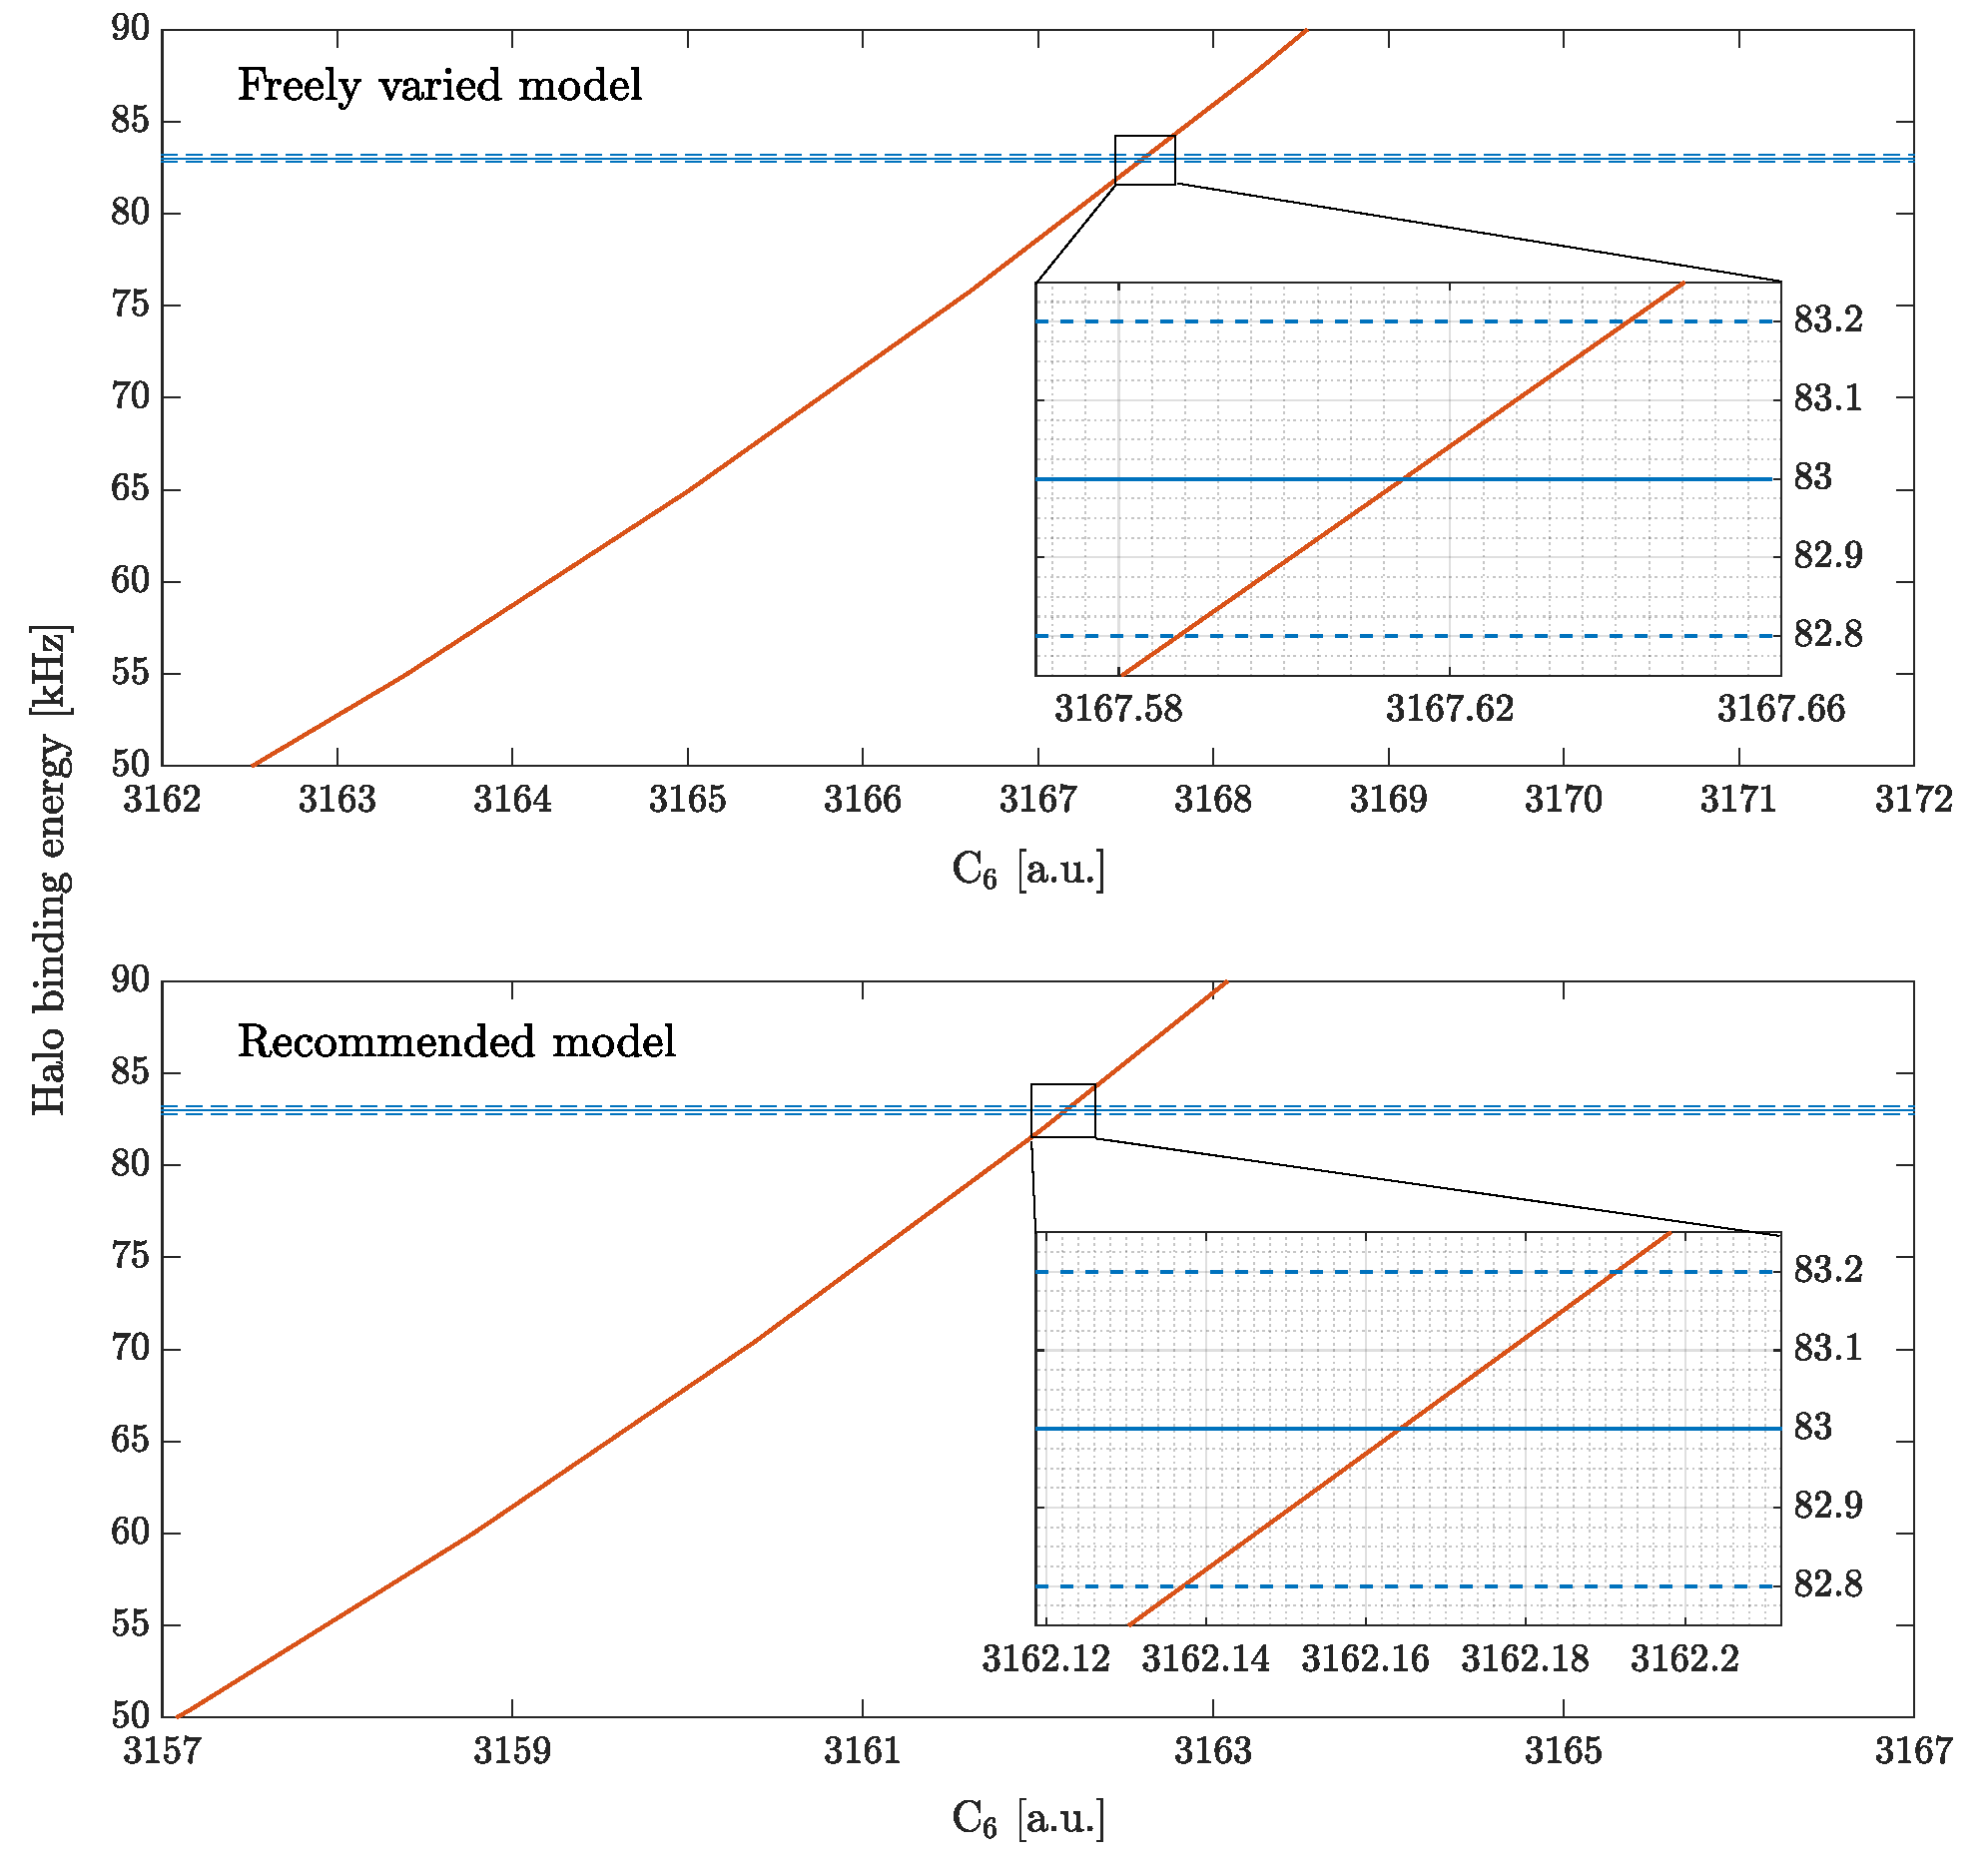
\includegraphics[width=\textwidth]{compOfC6.pdf}}
	  \caption{Comparison of C$_6$ coefficient estimates}{The $^{86}$Sr halo state binding energy is calculated using Eq.\,\ref{Eq:BindingEnergyGao} and numerical integration of the piece-wise potentials from Stein et al. (2010) \cite{Stein2010}. Comparing the measured halo state binding energy to these predictions gives an estimate of the underlying $C_6$ underlying value.}
	  \label{fig:c6estimates}
	\end{figure}
From these plots we can determine a $C_6$ value for each form of the potential.
However, the precision of our measurement exceeds that of either model and suggests that this work could be useful to further develop a theoretical understanding of the long-range portion of the strontium X$^1\Sigma_g^+$ potential since the halo state should be incredibly sensitive to the value of $C_6$.
Table \ref{tab:c6comp} shows all published values, and errors where available, for this $C_6$ coefficient.
We have included both of our values for completeness and show that they are in agreement with a majority of the published literature.
\begin{table}[]
\centering
\resizebox{\textwidth}{!}{%
\begin{tabular}{lll}
$C_6$ [a.u.] & Reference & Type \\ \hline
$3212$ & Stanton (1994) \cite{Stanton1994} & Theory \\
$3170\pm197$ & Porsev et al.\,(2002) \cite{Porsev2002} & Theory \\
$3249$ & Mitroy et al.\,(2003) \cite{mbr03} & Theory \\
$3131\pm41$ & Lima et al.\,(2005) \cite{Lima2005} & Theory \\
$3103\pm7$ & Porsev et al.\,(2006) \cite{Porsev2006} & Theory \\
$3130\pm20$ & Martinez de Escobar et al.\,(2008) \cite{MartinezDeEscobar2008} & Experiment \\
$3164\pm10$ & Stein et al.\,(2010) \cite{Stein2010} & Experiment \\
$3142$ & Skomorowski et al.\,(2012) \cite{Skomorowski2012} & Theory \\
$3107\pm30$ & Zhang et al.\,(2014) \cite{zbb14} & Theory \\
\begin{tabular}[c]{@{}l@{}}$3162.16\pm0.03$ - Freely varied\\ $3167.61\pm0.03$ - Recommended\end{tabular} & Aman et al.\,(2018) \cite{Aman2018} & Experiment
\end{tabular}%
}
\caption{Comparison of $C_6$ values from literature}{All values are given in atomic units. Note that the uncertainty of the present measurement reflects the uncertainty in the binding energy of the halo molecule.}
\label{tab:c6comp}
\end{table}
The quoted $C_6$ values are found from Fig.\,\ref{fig:c6estimates} by applying a linear fit, in the region of the binding energy, to the $C_6$ curves.
From these fits we find the intersection of $C_6$ and the binding energies at $83 \pm 0.2$\,kHz for both models.

Interestingly, despite our estimated values for $C_6$ being model dependent, the calculated scattering lengths from each model are found to be nearly identical, differing by $< 0.5$\% across all isotopes.
Fig.\,\ref{fig:massScaling} gives the mass-scaled scattering lengths for all strontium isotope combinations.
	\begin{figure} 
	\centerline{
	  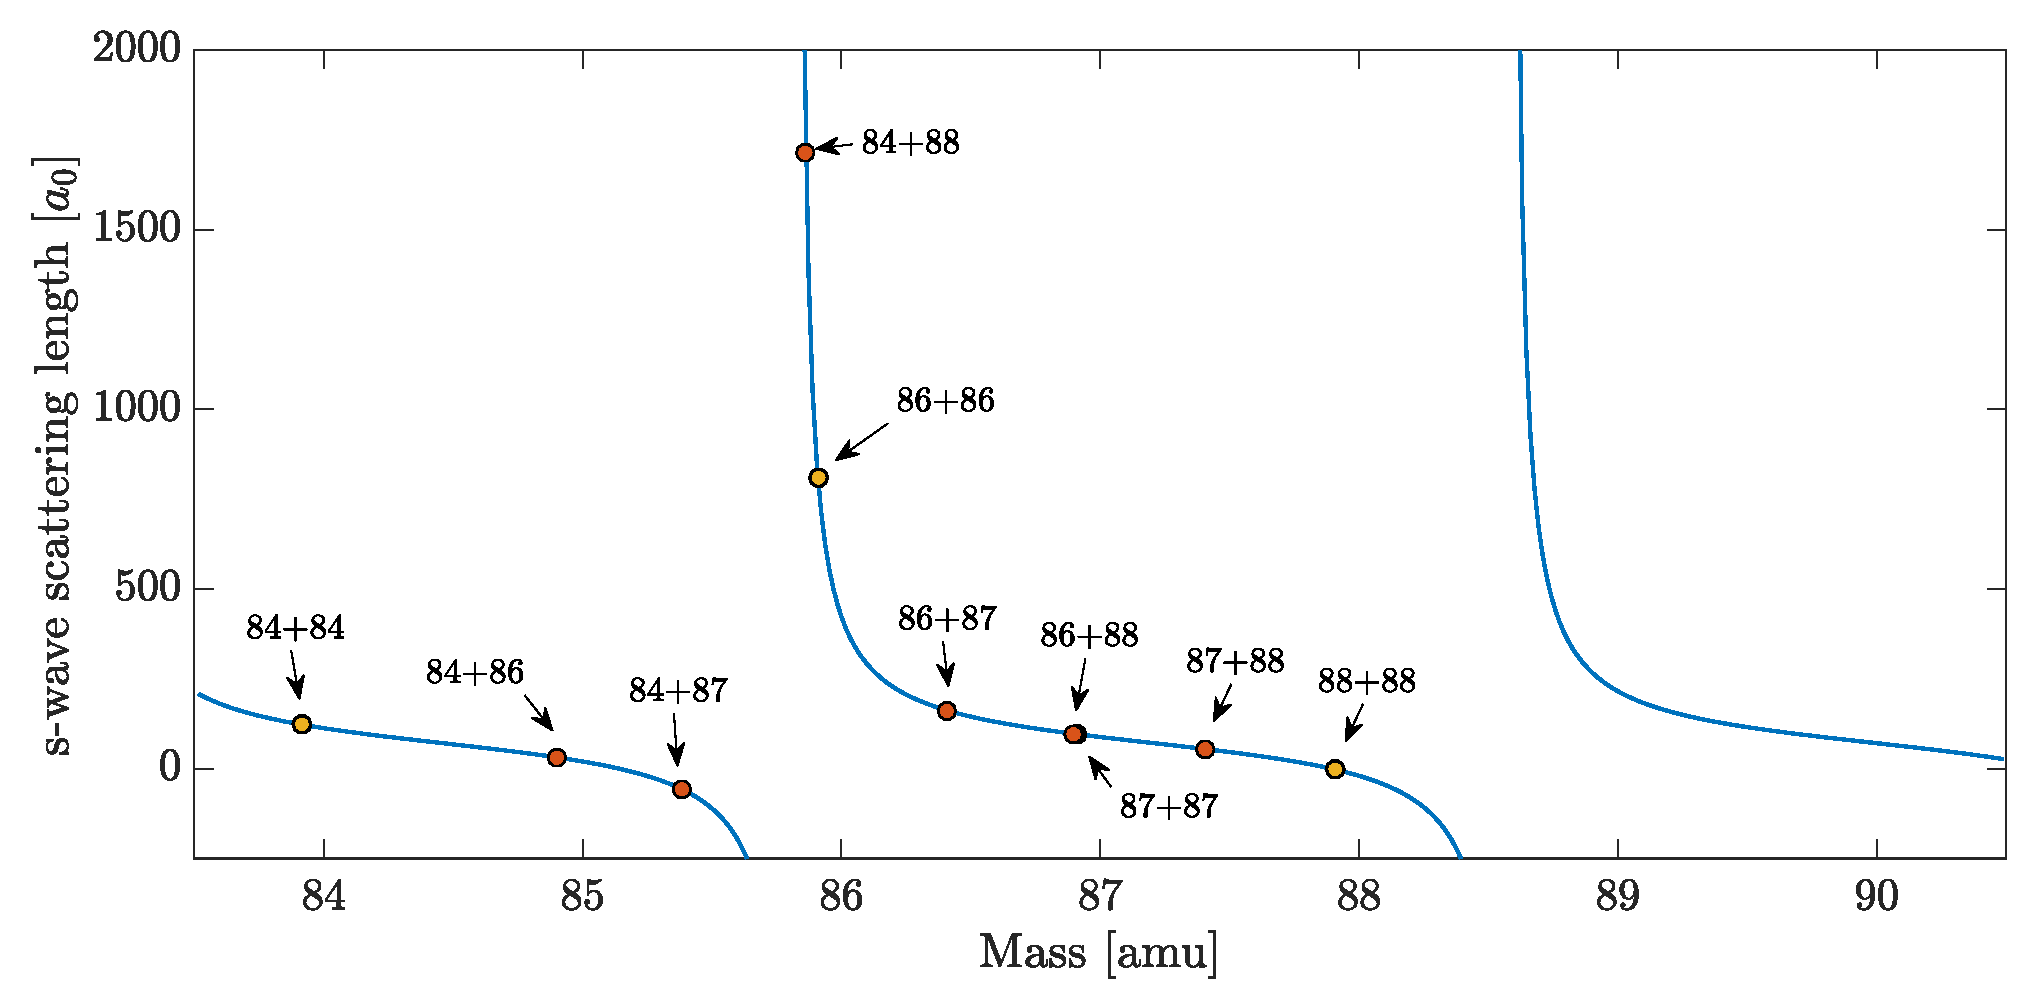
\includegraphics[width=\textwidth]{massScalingWithTable.pdf}}
	  \caption{Estimation of scattering lengths via mass scaling}{}
	  \label{fig:massScaling}
	\end{figure}
The quoted values of $a$ are found using the two different models, each with the their appropriate value of $C_6$ as given in Table \ref{tab:c6comp}.
These $C_6$ estimates are used to construct and numerically integrate the potential from $R_i\rightarrow\infty$ according to Eq.\,\ref{eq:5scatterLeng}, where $R_i=7.5$\,a$_0$ is the inner turning point of both models.
Finally, taking the value and error estimates from both models the quoted scattering length is the average of the values from either model and the uncertainty is the quadrature sum of the error from each model.


%% paper

%The properties of halo molecules have been well studied \hl{\cite{Kohler2006}}.
%One of the most interesting features is their universality, meaning that in the extreme, they can be characterized by a single parameter, the $s$-wave scattering length. For example,


%% %% %% %% %% %% %% %% %% %% %% %% %% %% %% %% %% %% %% %% %% %% %% %% %% %% %% %% %% %% %% %% %% %% %% %% %% %% %% %% %% %% %% %% %% %% %% %% 
%% other thoughts
%From the formula for the line shape we can see that it depends on the spatial distribution of the atoms.
%
%The standard approximation made when measuring these types of systems is to ensure loss does not cause heating of the atoms during photoassociation. 
%
%Heating results in re-equilibration of the atomic density distribition, which in turn effects the rate of loss creation. 
%
%Without independent controls to keep the system in thermal (and therefore spatial density) equlibrium.
%
%What are the things the rate equation deals with?
%
%We need the desnity distribution.
%
%In a harmonic trap, there if a simp[le anayltic form to the density distribution of a thermal gas. 
%
%
%From Mi's work (and others) we know that this is only an approximation that is valid when eta is approx greater than 4. 
%
%When greater than 4 we can apply the high-eta approx and the trap frequencies along a particular direction reduce to <eq>.
%
%However, the trap we did this experiment in were at eta's of 1 or less so we don't have an analytic solution to the spatial distribution.
%
%Since this could be a problem we need to know what the trap looks like.
%
%We measure trap oscillation freq. at several different powers and model the trap using the utility outlined somewhere else.
%
%From the numeric model, we can define a spatially depedent eta which is determined by the local trap depth which is simply the difference between the local potential energy and the global depth.
%This is illustrated in fig something.
%
%The spatial information is not only important for the density determination, but also for the range of available thermal energies.
%
%Consider two atoms near the local bottom of the trap. By definition, in equilibrium, a single atom may only have up to the trap depths worth of energy since any additional energy would result in its expulsion from the trap.
%
%In this case, in a relative momentum frame, the allowed collision energies range from zero to two times the trap depth.
%
%Similarly, as we move towards the edge of the trap the range of accessible collision energies shrinks.
%
%Normally the BZ dist goes to infinity but here we have a cutoff at 2 trap depeth.
%The most naive approx would be to simply consider the BZ and harshly truncate at 2 trap depth. We tried this
%
%We know this is unphysical since we should expect that the probability of observing a certain momenta at a certain point in space, should smoothly tend zero towards as we approach the edge of the trap.
%To see what this looks like we (and determine how important the effect is) we rederive the relative momentum distribution.
%
%<Some stuff about center-of-mass and relative>
%
%What were all the cases and conclusions of having done this? Remember to consider what the different cases are.
%
%If the total relative energy can be X then how does that get split up? Use the plots to show this limiting behavior.
%
%Like if particle 1 has all the energy then there is only one possible value for particle 2 (and vice versa).
%
%DERIVATION for truncated trap below
%
%Need to lookup references for this molecular chaos assumption. What about egodicity? How to discuss that we may not be completely ergodic?
%
%What does my potential look like? Can I make it a piecewise function? How should I introduce this part?
%
%Where does the f equation come from? I believe this is just the normalized boltzmann factor for probability to occupy a particlar state.

%\noindent
%We can truncate this single particle distribution by 
%\begin{equation}
%\label{eq:trun_single_particle_prob}
%		 f_{ \vec{r} }( \vec{p} ) = A \left(\frac{1}{2 \pi k_B T}\right)^{3/2} e^{\left(\frac{-p^2}{2 m k_B T}\right)} \Theta \left( \epsilon_{max} - U( \vec{r} ) - \frac{p^2}{2 m} \right)
%\end{equation}
%
%\noindent
%where A is a normalization constant which ensures $\int_0^\infty f_{ \vec{r} }( \vec{p} )\,d \vec{p} = 1 $ and $\Theta(x)$ is the Heaviside function defined by
%
%\begin{equation}
%\label{eq:heaviside}
%	\Theta(x)=
%	\begin{cases}
%		1 &\text{if } x \geq 0, \\
%		0 &\text{if } x < 0
%	\end{cases}
%\end{equation}
%
%We got a certain answer with the way shown in the paper.
%
%We can also use a completely different method that ignores all the consdierations of the last few sections. As was done in the calcium paper, we could simply fit the blue edge of the feature using a model function which can capture the high level features of the lineshape. Get the same answer. SHOW PLOTS TO THIS AFFECT AND COMPARE
%
%Maybe go a little into the isolated resonance model (or at least recall), then tie into how we can measure the susceptibility across several different detunings which can give us the coupling to intermediate level. The first order analysis of this data suggest a bound-bound rabi freuqnecy of \hl{BLAH}. 
%
%Point out the curling up at the end and say how the simple isolated resonacne model cannot predict.
%
%A full coupled channel calculation probably could but in the spirit of the Bohn and Julienne semi-classical approach, we set out to derive an approximate analytic expression to determine the binding energies.
%%
%THis is presented in the next chapter.
%
%Lastly, we note that in the context of photoassociation, the center-of-mass component of Eq.\ref{eq:two_particle_prob_inf_atomFrame} is not typically considered as typical PAS experiments are performed utilizing broad dipole allowed transitions which have linewidhts much greater than the doppler width thus only the relative momentum between particles is important for determining the loss rate coefficient K discussed in \hl(somewhere). 
%
%The case of PA using narrow intercombination line transitions found in alkaline-earth-metal atoms 
%
%In general K is considered as a boltzmann average over a single loss rate constant
%This can be seen in \hl{\cite{Ciuryo2004}} Eq. 1 where the loss rate constant is given by
%
%\begin{equation}
%\begin{split}
%\label{eq:ciuryo04_eq1}
%		 K(\Delta,T) &= \left\langle\mathcal{K}(\Delta,\vec{P}_c,\vec{p}_r)\right\rangle \\
%		 &= \int d^3\vec{P}_c \; f_M(\vec{P}_c) \int d^3\vec{p}_r \; f_{\mu}(\vec{p}_r) \; \mathcal{K}(\Delta,\vec{P}_c,\vec{p}_r)
%\end{split}
%\end{equation}


%To this end we can integrate out the center-of-mass component to obtain the distribution most typically relevant to photoassociation.
%
%By the time I've gotten to this I have already introduced K and that is not what I wanted to do. 
%
%conclusion
%here is the modified version of K we need for a trap that has a truncated energy disttribution
%
%to get there
%normal version of K is \hl{given in ch3}
%this K can be given in terms of f? 
%this version of f is given in the appendix
%	why do I integrate out the com component?
%
%typical PAS experiments utilize dipole allowed transitions which have linewidths many times larger than the 
%
%We now perform a change of variables using Eq. and Eq.\ref{eq:two_particle_prob} can be rewritten as 
%
%In the $s$-wave limit I need to write K as a function of f(p) (should do this in the appendix proof and reference in body). Given the form of the loss rate constant K, our problem reduces to determining the form of f(p) when eta is finite.
%
%Ok, so need to reference \hl{\cite{Ciuryo2004}} to motivate usage of center-of-mass.
%Then use \hl{\cite{Nicholson2015a}} Eq. 43 to reference the particular form 
%
%
%what is the throughline I want to make? Develop K$_{in}$ $\rightarrow$ recast in terms of P distribution $\rightarrow$ show how we can replace the normal dist with a truncated dist $\rightarrow$ explore the effects of that truncation 


%To prove this assumption I want to show that using the square step I can get the same equations like in Eq. 1 of the 99 paper. Then once we know the infinite energy behavior (valid for only a particular portion of energy due to $s$-wave constraint) then we can ask what happens if f(p) is truncated. 


%The long-range form of the interaction for $s$-wave collisions, which determines many aspects of atomic scattering at ultracold temperatures,  can be described with a van der Waals form, $V(r)=-C_6/r^6$. %where $C_6=3.03(1) \times 10^{-76} J m^6$  for Sr \hl{\cite{Stein2010}}.
%Details of low energy scattering and near-threshold states for  a van der Waals potential have been well studied, and an important length scale was defined in \hl{\cite{gfl93}} as the mean scattering length or interaction range \hl{\cite{cju05}}
%\begin{equation}\label{Eq:InteractionRangevdW}
%  \bar{a}=2^{-3/2}\frac{\Gamma\left(\frac{3}{4}\right)}{\Gamma\left(\frac{5}{4}\right)}\left(\frac{2\mu C_6}{\hbar^2}\right)^{1/4},
%\end{equation}
%where $\mu$ is the reduced mass  and $\hbar$ is the reduced Planck's constant.
%$C_6=3.03(1) \times 10^{-76} J m^6$ \hl{\cite{Stein2010}} and
%, where $a_0=5.29\times 10^{-11}$\,m is the Bohr radius.
%This value of $C_6$ is consistent with a recent \textit{ab initio} calculation \hl{\cite{zbb14}}.
%\begin{equation}\label{Eq:InteractionRangevdW}
%  \bar{a}=2^{-3/2}\frac{\Gamma\left(\frac{3}{4}\right)}{\Gamma\left(\frac{5}{4}\right)}\left(\frac{2\mu C_6}{\hbar^2}\right)^{1/4}.
%\end{equation}
%The universal relation $E_b=-\hbar^2/2\mu a^2$ is valid in general very close to a scattering resonance and over all values of scattering length for a zero-range delta-function pseudopotential .
%\begin{equation}\label{Eq:HaloEnergyLeadingCorrection}
%-\hbar^2/2\mu(a-\bar{a})^2.
%\end{equation}
% This expression has been shown to be accurate for numerous magnetic Feshbach resonances \hl{\cite{Chin2010,Kohler2006}}, such as in $^{85}$Rb \hl{\cite{kgb03,ckt03}}.
%Higher order corrections due to
